
\includegraphics[height=1.25cm]{images/pictograms/replication}
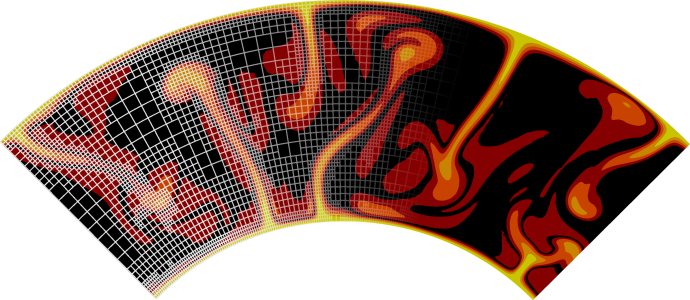
\includegraphics[height=1.25cm]{images/pictograms/aspect_logo}

\includegraphics[height=1.25cm]{images/pictograms/benchmark}
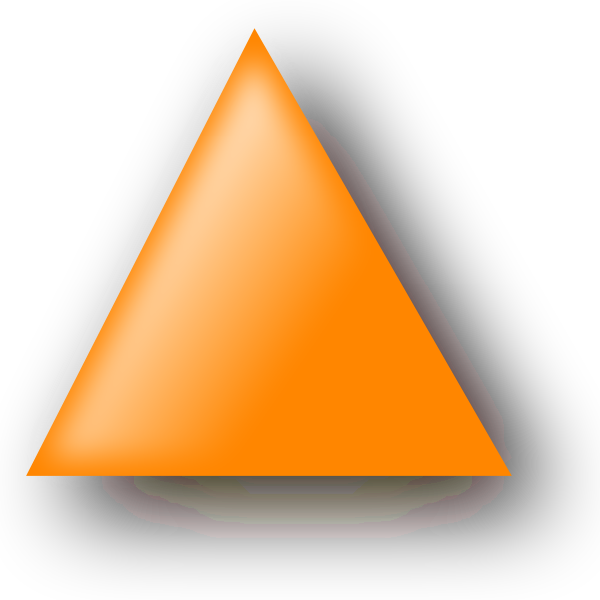
\includegraphics[height=1.25cm]{images/pictograms/triangle}

\includegraphics[height=1.25cm]{images/pictograms/FEM}

%%%%%%%%%%%%%%%%%%%%%%%%%%%%%%%%%%%%%%%%%%%%%%%%%%%%%%%%%%%%%%%%%%%%%%%%%%%%%%%%%%%%%%%%%%%%%%%%%%%

\begin{flushright} {\tiny {\color{gray} python\_codes/fieldstone\_142/text.tex}} \end{flushright}

\lstinputlisting[language=bash,basicstyle=\small]{python_codes/fieldstone_142/keywords.key}

\begin{center}
\fbox{\textbf{\huge \color{teal} P}}
Code at \url{https://github.com/cedrict/fieldstone/tree/master/python_codes/fieldstone_142}
\end{center}

\par\noindent\rule{\textwidth}{0.4pt}
%%%%%%%%%%%%%%%%%%%%%%%%%%%%%%%%%%%%%%%%%%%%%%%%%%%%%%%%%%%%%%%%%%%%%%%%%%%%%%%%%%%%%%%%%%%%%%

This \stone is based on \textcite{hams22} (2022) published in the Journal of Structural Geology.
As for every \stone aiming at reproducing results off a publication I here include de abstract
of the article:

\begin{center}
\begin{minipage}{13cm}
{\small 
Computer-based numerical solutions of geomechanical problems are important to understand the processes
forming rock structures as well as to quantify the associated pressure, stresses and strain rates. However, the
development of such computer programs and the underlying mathematical methods are commonly not taught in
a standard structural geology curriculum. Here, we present a simple computer program to calculate the stress,
pressure, velocity and strain rate fields for two-dimensional (2D) viscous inclusion-matrix systems under pure
shear and simple shear. The main aim of our contribution is to explain this computer program in a simple and
transparent way, so that it can be used for introductory courses on geomechanical numerical modelling in
structural geology. We present the governing equations of 2D viscous deformation and program the equations in
the same order and style, so that the equations are still recognizable in the computer program. The computer
program can treat stiff and weak inclusions of any shape and considers both linear and power-law viscous flow
laws. We present numerical calculations for various inclusion-matrix scenarios. The program is written with the
software MATLAB, is provided as supplementary material, and can also be run with the freely available software
GNU Octave.}
\end{minipage}
\end{center}
 

In the paper the effective viscosity for a power-law viscous fluid, termed here $\eta_{PL}$, can be written
as
\[
\eta_{PL}=\eta_L \left( \frac{\tau_e}{\tau_R}  \right)^{1-n}
\]
where $\eta_L$ is the linear viscosity, $\tau_R$ is a constant reference stress, 
$n$ is the stress exponent (which for rocks is $\ge$1), and $\tau_e$ is the effective 
deviatoric stress.

Often, a combination of linear viscous and power-law viscous flow is
assumed for ductile rocks. The viscosity for such combined flow law can
be given by the pseudo-harmonic mean of $\eta_L$ and $\eta_{PL}$:
\[
\eta_C = \left(  \frac{1}{\eta_L} + \frac{1}{\eta_{PL}} \right)^{-1}
\]
The effective viscosity, $\eta$ in the momentum conservation equation can, hence, either be
equal to $\eta_L$, $\eta_{PL}$ or $\eta_C$ depending on whether a linear viscous, power-law
viscous or combined flow law, respectively, is used.

The paper relies on the Finite Difference method to solve the Stokes equations but we will here 
rely on the Finite Element method based on an unstructured mesh.

\begin{center}
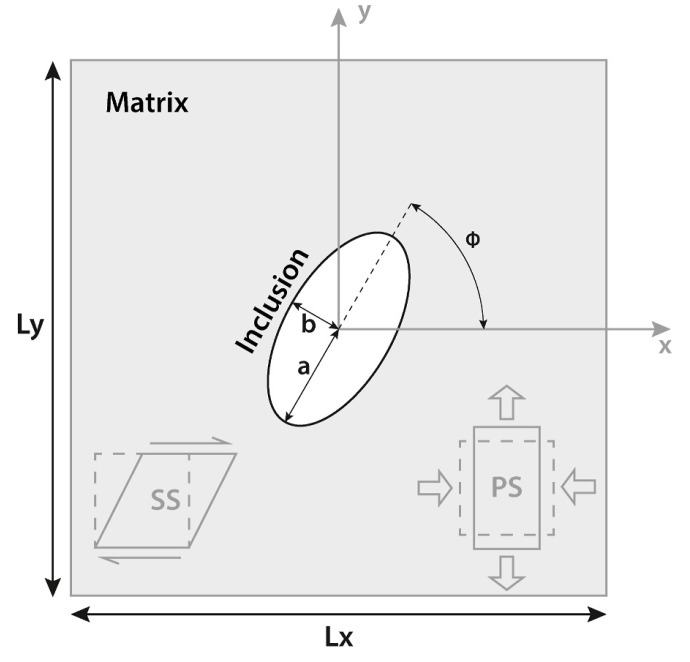
\includegraphics[width=6cm]{python_codes/fieldstone_142/images/hams22_a}\\
\captionfont{Taken from \cite{hams22}.
Model configuration and boundary conditions. An elliptical inclusion of
different viscosity than its surrounding matrix is located in the center of a
square box of size Lx by Ly. The ellipse has a semi-major axis $a$ and semi-minor
axis $b$ and is rotated by angle $\phi$ from the horizontal axis. Both simple (SS) and
pure (PS) shear boundary conditions can be applied.}
\end{center}

Boundary conditions are either a far-field pure shear velocity field at the model boundaries
or a simple shear velocity field.
Hence, both the horizontal and vertical components of the velocity are defined as
boundary conditions at the model boundaries.

The model domain consists of a matrix in which stiffer or weaker inclusions are embedded. As
initial guess for the unknown velocities, which is required for the first
iteration step, the authors assume that the velocity field in the model domain
corresponds to either a homogeneous pure shear or homogeneous simple
shear velocity field, depending which far-field velocity boundary conditions are applied. 

%----------------------------------------
\subsection*{Comments about the article}

A few remarks:
\begin{itemize}
\item The authors also state that ``The pressure values at the model boundaries remain zero.'' uh??!
\item The viscosity field is smoothed but this is never mentioned in the paper!
\begin{verbatim}
for smo=1:2; Ii  = [2:nx-1]; Ij  = [2:ny-1]; % Smoothing of the initial viscosity field
    ETA(Ii,:)    = ETA(Ii,:) + 0.4*(ETA(Ii+1,:)-2*ETA(Ii,:)+ETA(Ii-1,:));
    ETA(:,Ij)    = ETA(:,Ij) + 0.4*(ETA(:,Ij+1)-2*ETA(:,Ij)+ETA(:,Ij-1));
end
\end{verbatim}
This looks like a discretised diffusion operator...

\item no real benchmarking, no error convergence on SolVi, instead: instead eyeball norm
\item no solver in code ... why use Richardson rather than backslah operator of matlab? This finally explained in Discussion but
this should have been addressed earlier in the paper since it is rather uncommon.  
\item no comment on viscous relaxation in fig 7 ?
\begin{verbatim}
ETA_PL = exp(log(ETA_PL)*0.5+log(ETA_PL_it)*0.5);
\end{verbatim}
 
\item in the Octave code:
\begin{verbatim}
subplot(224),pcolor(X,Y,DXX/(2*eta_B*D_B)),shading interp,axis equal,axis tight,colorbar,colormap(jet)
         title(['D) Horizontal strain rate [ ], D_{xx}/D_B']), xlabel('Width [ ]')
\end{verbatim}
We see that there is a mismatch between what is plotted and the legend (\verb|DXX/(2*eta_B*D_B)| vs. \verb|D_{xx}/D_B|)

\item As we will see in the ellipse inclusion case, the code fails to converge
for modest viscosity contrasts.

\item authors state: Considering more irregular geometries is important, 
because “the geometrical form of the competent
inclusion clearly has an influence on the pattern of stress orientations in the
surrounding medium”. Yet not a single stress or principal stress components calculations in the wole paper? 

\item Why are tensor notations not used ? (why eqs 1,2,3 and 4,5,6 ?)

\item 'spacial' ? 'quadratic model domain' ?

\item fig 5: why change the radius inside the figure? why viscosity contrast at 100, not 1000 ?

\item The provided code does not allow to reproduce experiments directly. Only ellipse. 

\item fig 9: resolution? applied velocity ? ``Except for the circular inclusion, all ellipses possess the same aspect ratio.'' Which is equal to ?

\item nothing about convergence pattern ? 1000's of iterations ? round off errors.

\item about fig 10: 'The value of Dxx inside the garnet inclusion is zero, indicating that the inclusion is rigid and not deforming.' 
No, Dxx cannot be and is not zero. 

\item in the corrigendum only ellipse figures are corrected, not all the other ones so that the figs in the paper are useless 
to us when it comes to nonlinear rheologies as they cannot be used for comparison/benchmarking.

\item often in figure captions: 'The arrows display the velocity field, they are not to scale and only for direction.'
However looking at the figures arrows have various lengths which reflect the velocity field.

\item in some plots, $Dxx$ is described as 'horizontal strain rate'. meh 

\end{itemize}


%----------------------------------------
\subsection*{Comments about the \stone}

The code solves the incompressible Stokes equations with the Finite Element Method
on an unstructured grid that is built so that it fits the shape of the inclusion(s).
$P_2\times P_1$ or Crouzeix-Raviart elements can be used.
The Delaunay triangulation is explained in \stone 131, and 
some of the tools are also used in \stone 96 and 143.
In what follows I focus only on the Newtonian cases.

I also make use of the \aspect code\footnote{\url{https://github.com/geodynamics/aspect}}
and the prm file is provided in results/case1/aspect. 

\newpage
%%%%%%%%%%%%%%%%%%%%%%%%%%%%%%%%%%%%%%%%%%%%%%%%%%%%%%%%%%%%%%%%%%%%%%%%%%%%%%%%%%%%%%%%%%5
\section*{Case 0: Circular inclusion and comparison with analytical solution}

The boundary conditions are pure shear extension.
This is the well known SolVi benchmark that has been already encountered in \stone 7,120.

\begin{center}
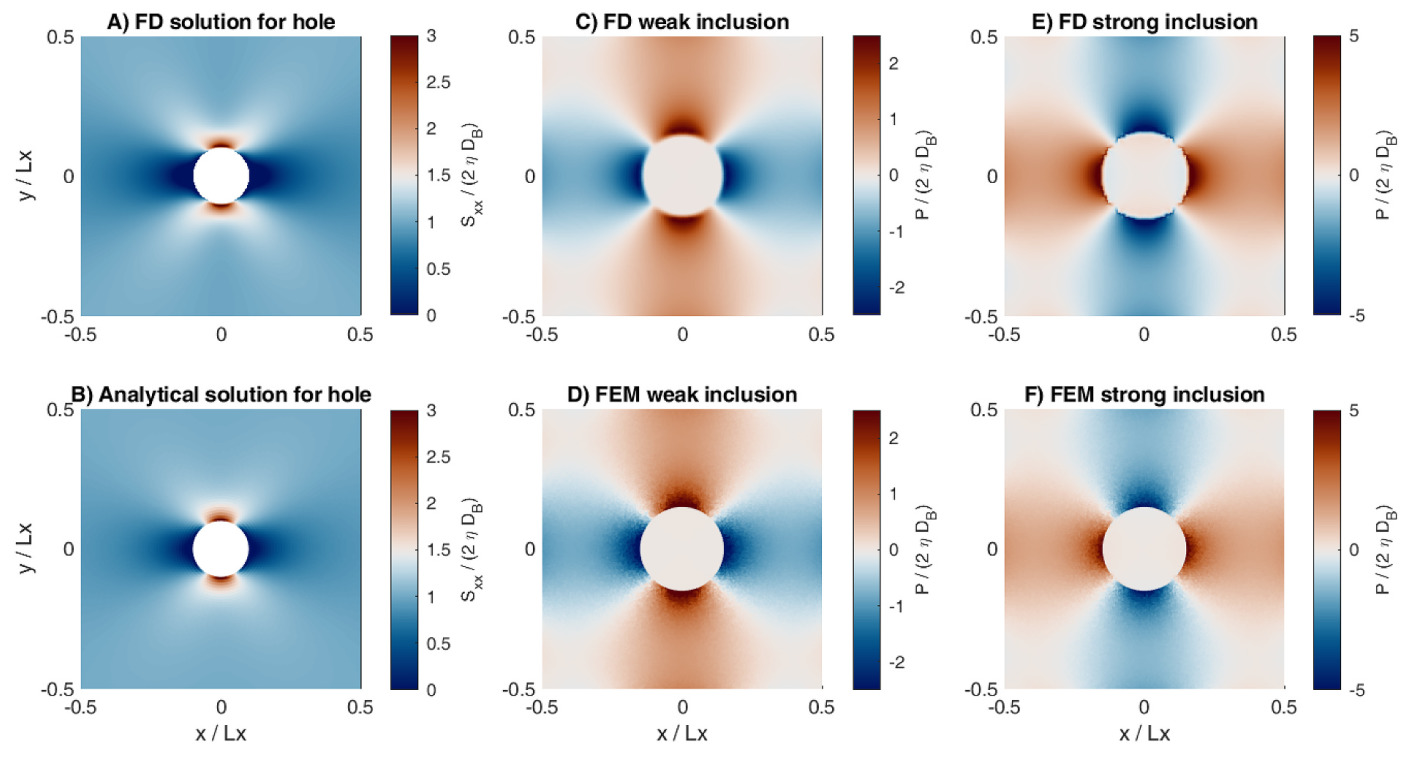
\includegraphics[width=12cm]{python_codes/fieldstone_142/images/hams22_b}\\
\captionfont{Taken from \cite{hams22}.
Panels A) and B): Comparison of the normalized horizontal total stress field generated with the presented iterative 
finite difference (FD) program against an analytical solution for a circular hole within a matrix subjected to 
horizontally extensional pure shear. The hole in the FD program is approximated by a viscosity
contrast of 1000. The hole radius is 0.1 times the model width. Panels C) to F): Comparison of 
the normalized pressure field generated with the presented iterative FD
program against a tested finite element method (FEM) program (Schmalholz and Schmid, 2012) for both a weak 
and a strong circular inclusion under horizontally compressive pure shear. The regions of high pressure (red color) 
and the low pressure (blue color) are inverted from the weak inclusion to the strong inclusion setup.
The viscosity of the inclusion is 100 times lower, respectively higher, than the surrounding matrix viscosity. 
The circle radius is 0.15 times the model width.}
\end{center}

\begin{center}
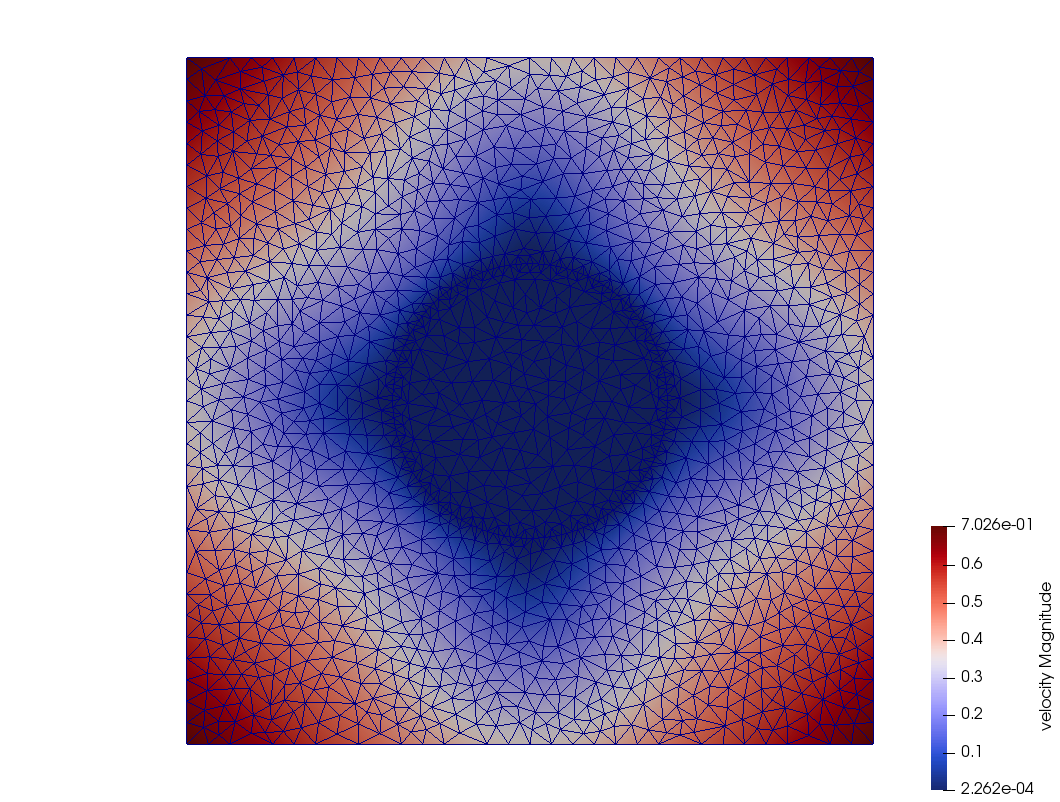
\includegraphics[width=5.7cm]{python_codes/fieldstone_142/results/case0/vel}
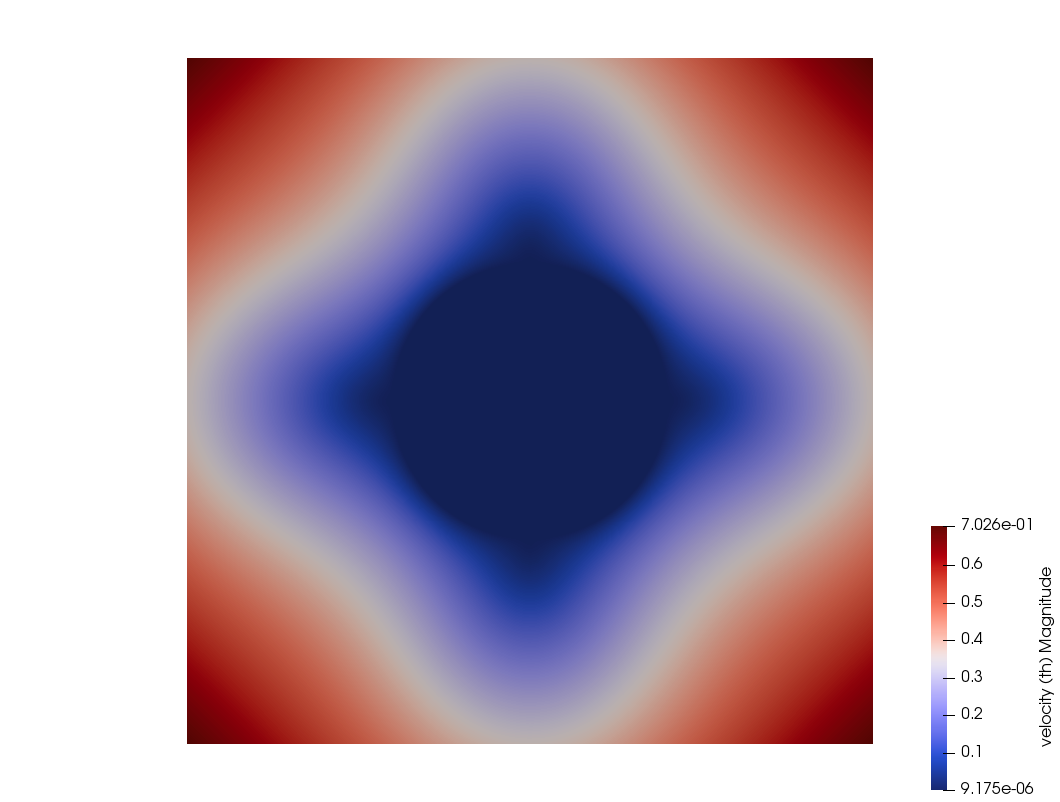
\includegraphics[width=5.7cm]{python_codes/fieldstone_142/results/case0/vel_th}\\
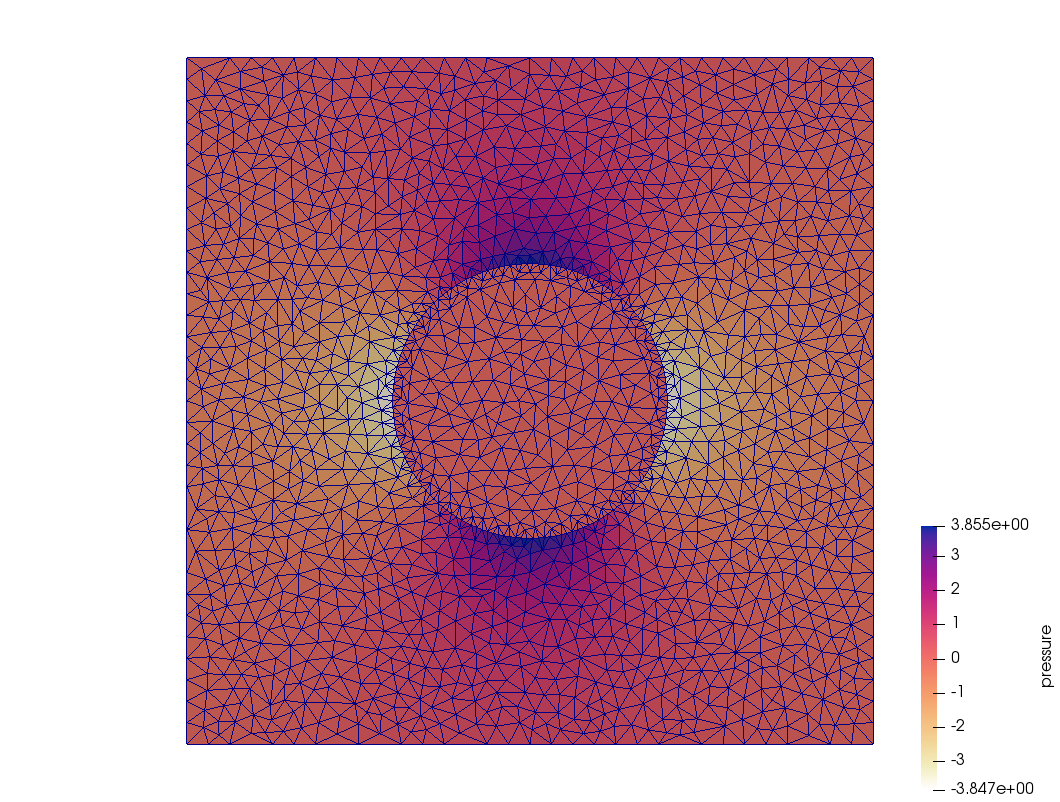
\includegraphics[width=5.7cm]{python_codes/fieldstone_142/results/case0/press}
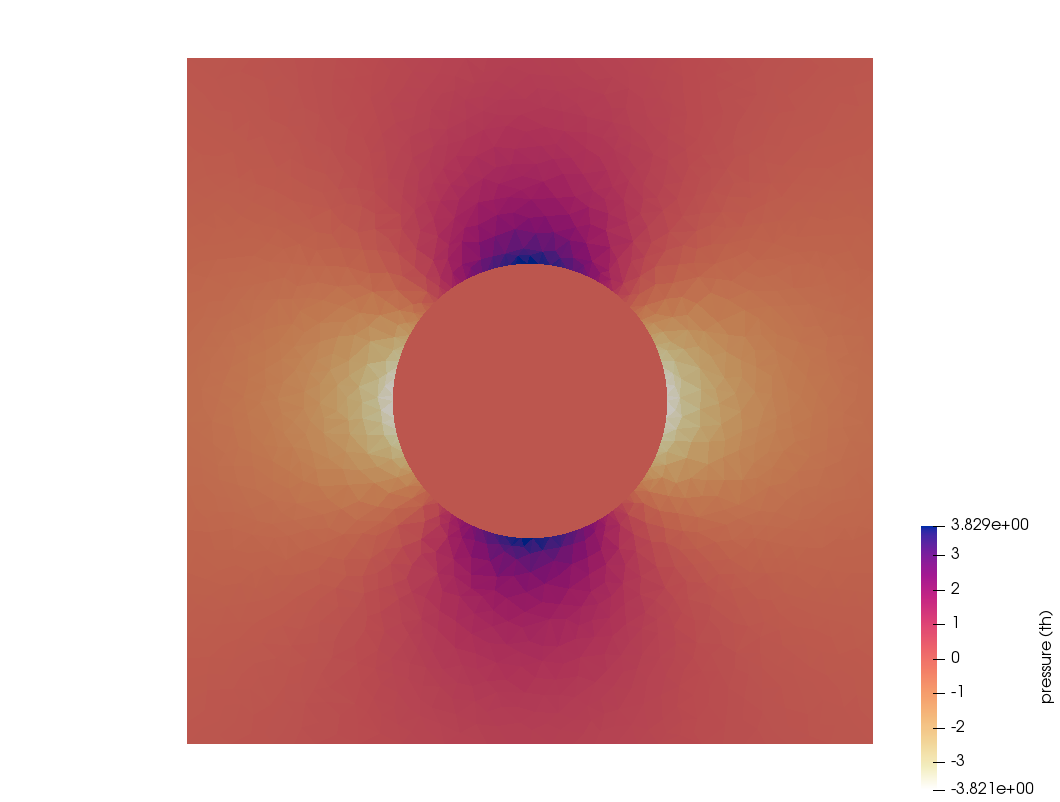
\includegraphics[width=5.7cm]{python_codes/fieldstone_142/results/case0/press_th}\\
{\captionfont Left: solution using Crouzeix-Raviart elements; Right: analytical solution.}
\end{center}

This proves that the code is correct. One should obviously do a proper error analysis as a function 
of resolution but this has been done before in many other stones (see \stone~\ref{f07} for example). 

\newpage
%%%%%%%%%%%%%%%%%%%%%%%%%%%%%%%%%%%%%%%%%%%%%%%%%%%%%%%%%%%%%%%%%%%%%%%%%%%%%%%%%%%%%%%%%%5
\section*{Case 1: Strong rectangular inclusion under pure shear and simple shear}

The authors state:
``For illustration purposes, we calculated the pressure fields for a strong and inclined rectangular 
inclusion for pure shear and simple shear. For simple shear, the
pressure variations are more localized around the inclusion compared to
the pressure variations for pure shear. Also, for simple shear the velocity
field indicates a rotational flow of the inclusion with a clock-wise sense,
in agreement with the applied simple shear.''

\begin{center}
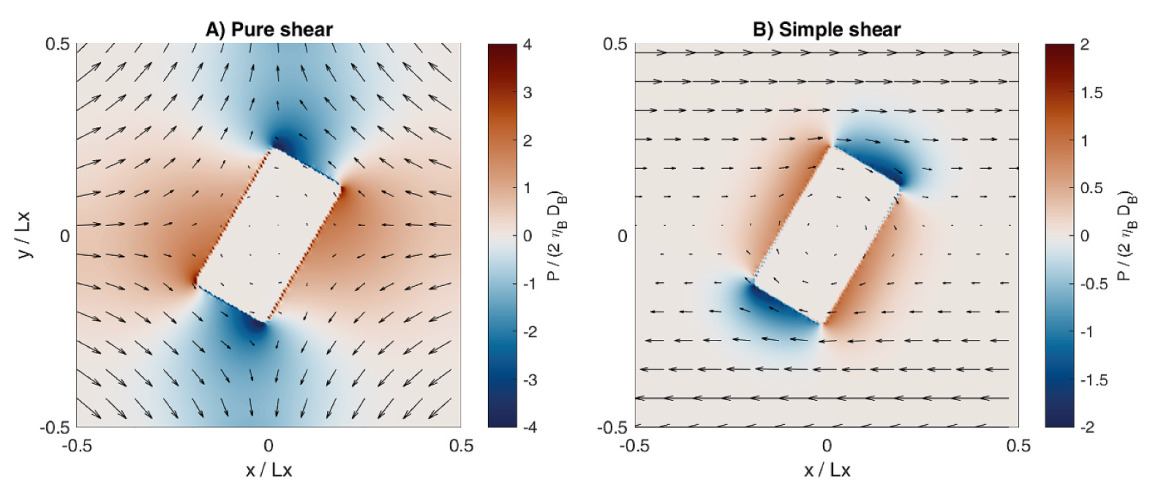
\includegraphics[width=13cm]{python_codes/fieldstone_142/images/hams22_c}\\
\captionfont{Taken from \cite{hams22}.
Comparison between horizontally
compressive pure shear and horizontal simple shear boundary conditions for a strong
(viscosity contrast of 1000) rectangular inclusion. Regions of pressure accumulation
are depicted in red, pressure shadow zones in blue. The arrows display the velocity field,
they are not to scale and only for direction. The long side of the rectangle is twice the 
size of its short side and corresponds to 0.4 times the model width. The long side of the
rectangle is rotated by an angle of 60 from the horizontal axis. }
\end{center}

\begin{center}
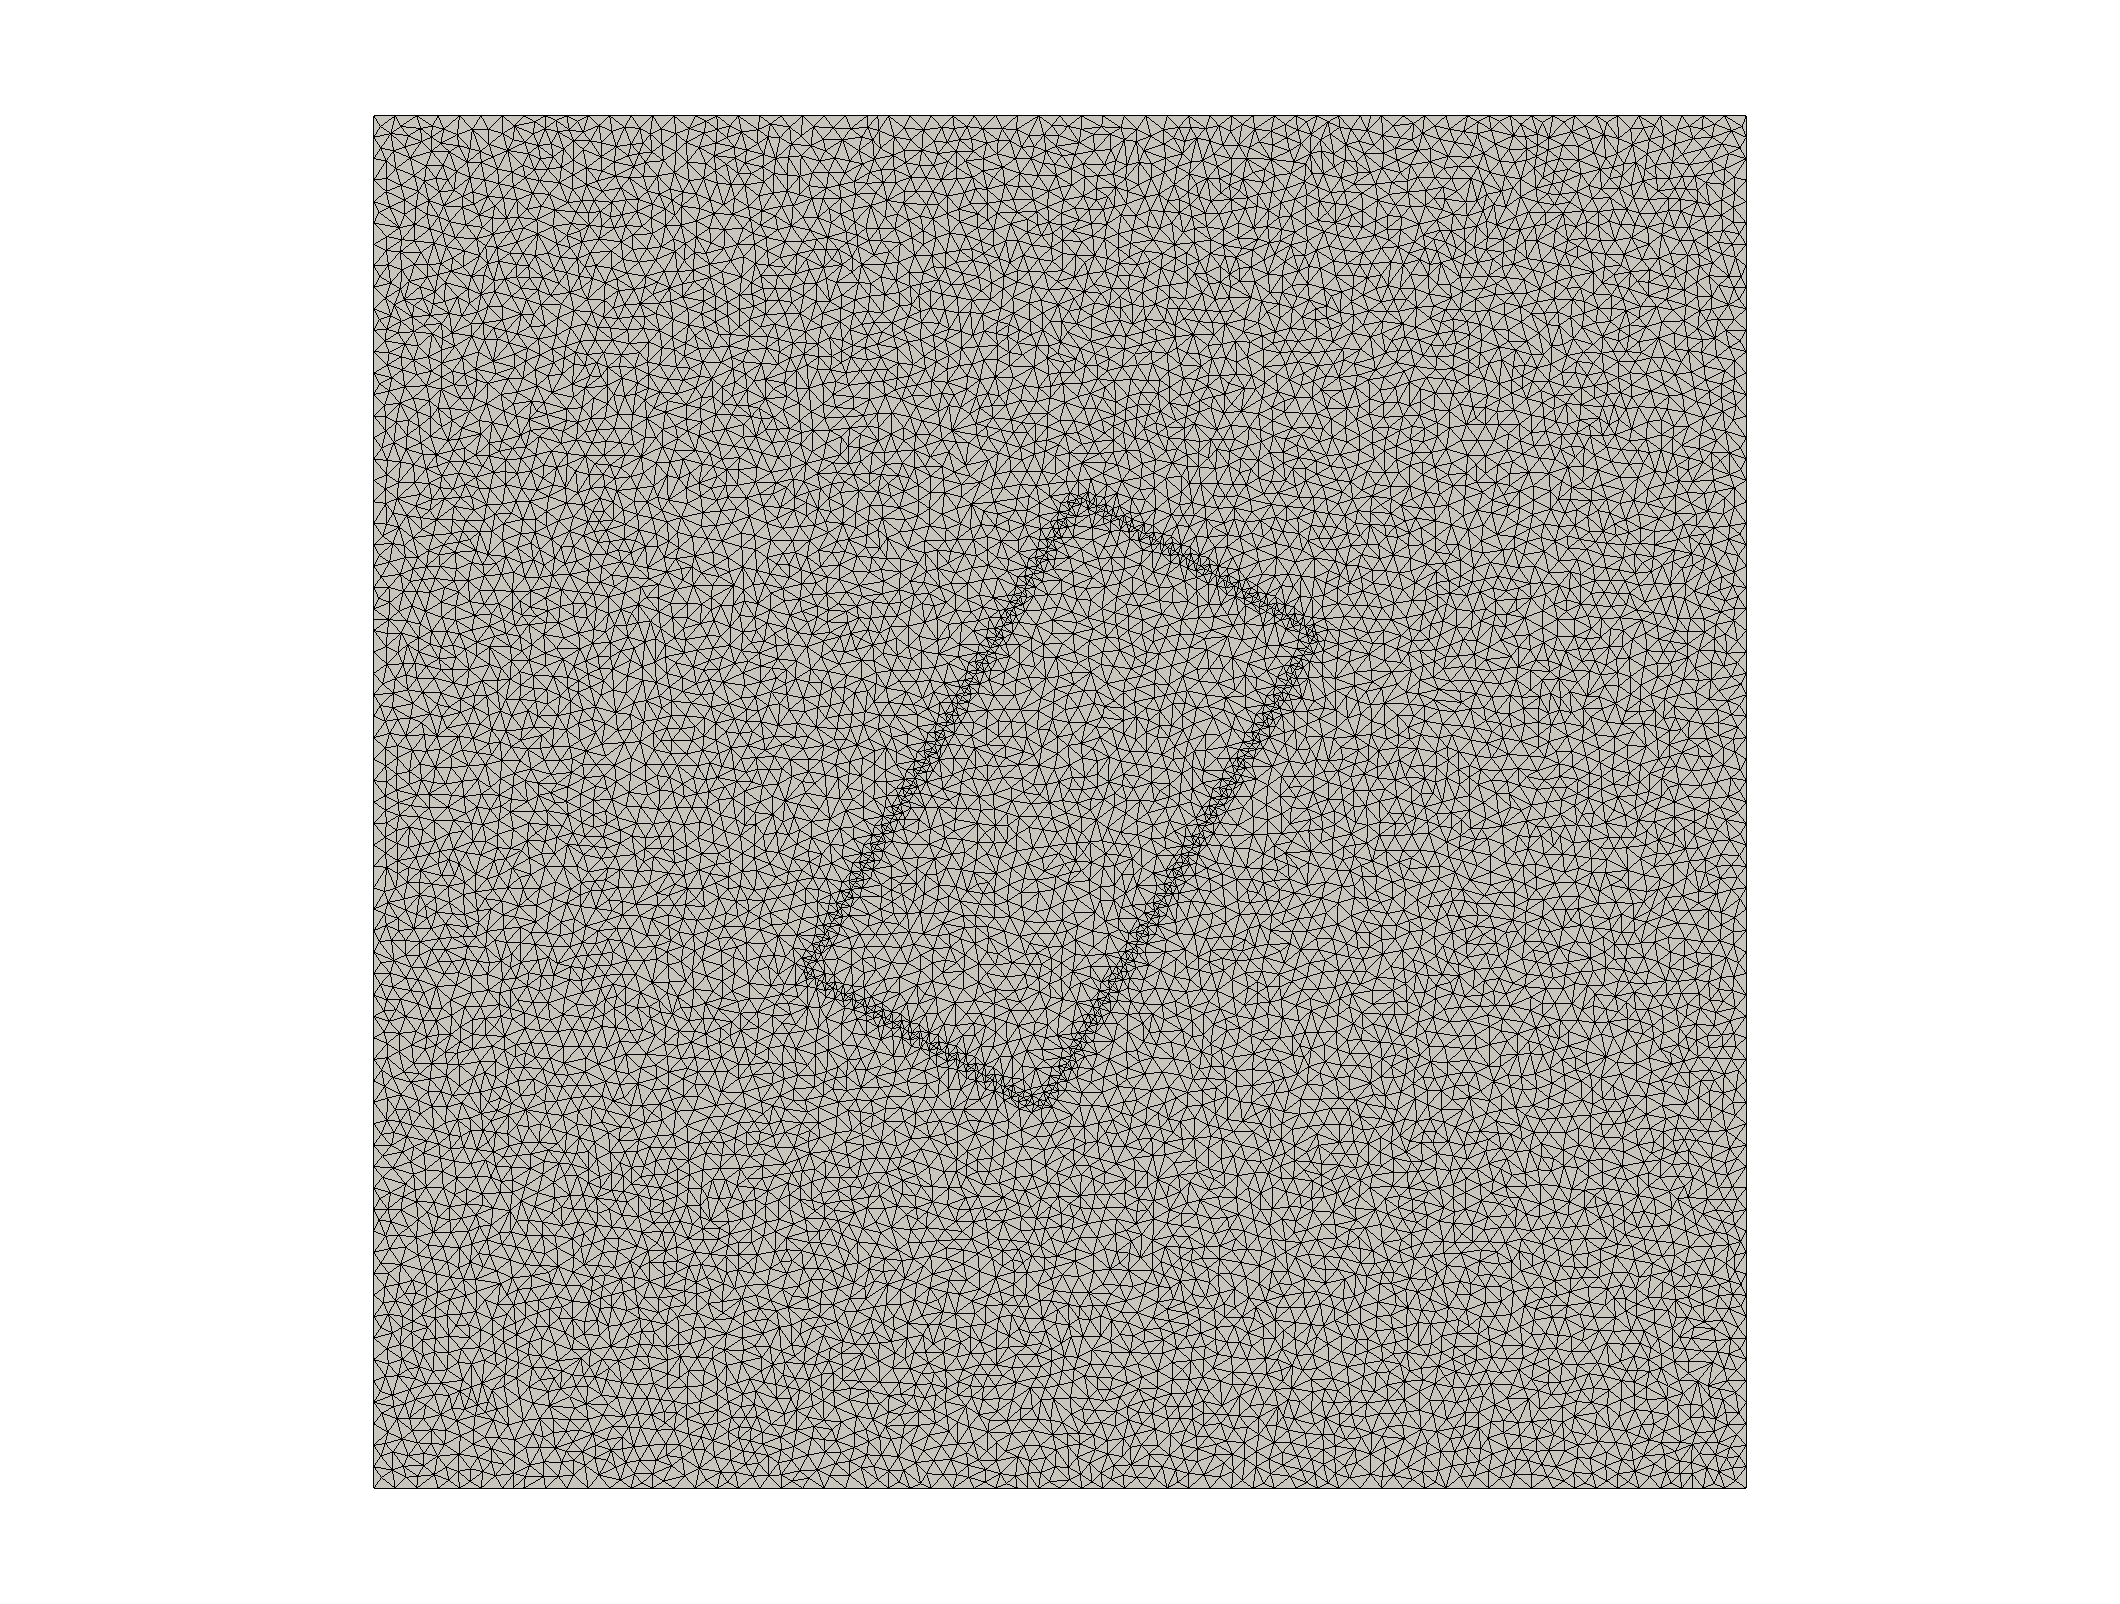
\includegraphics[width=5.57cm]{python_codes/fieldstone_142/results/case1/mesh}
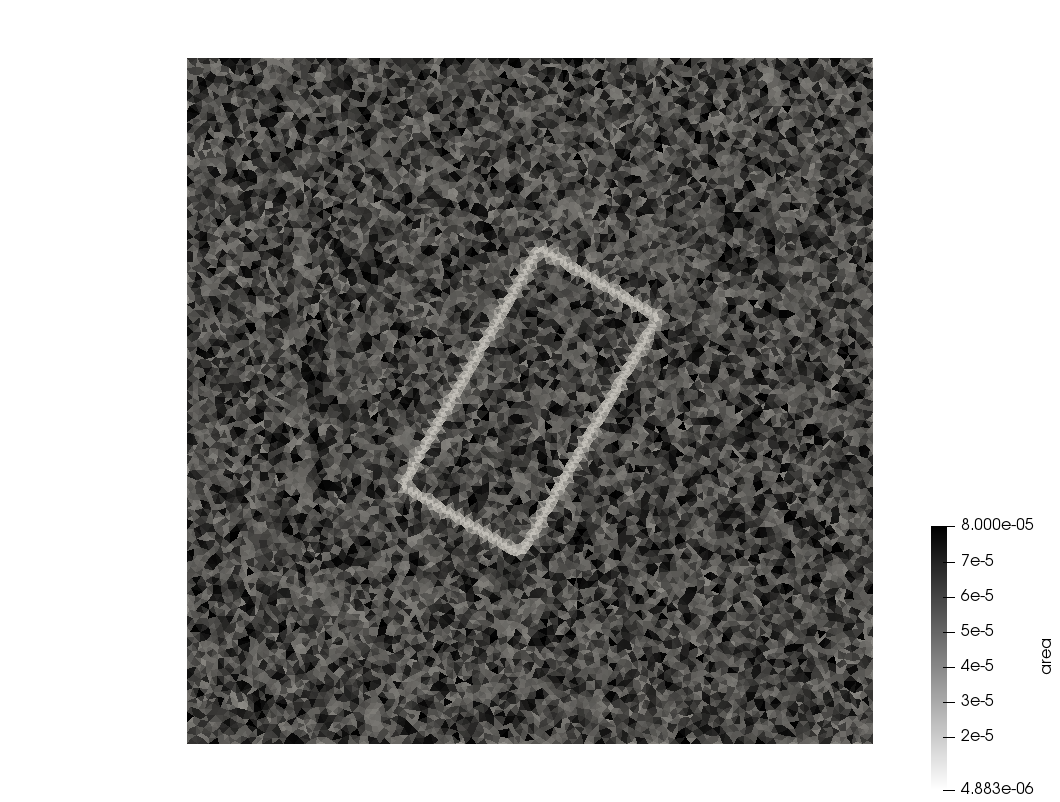
\includegraphics[width=5.57cm]{python_codes/fieldstone_142/results/case1/areas}
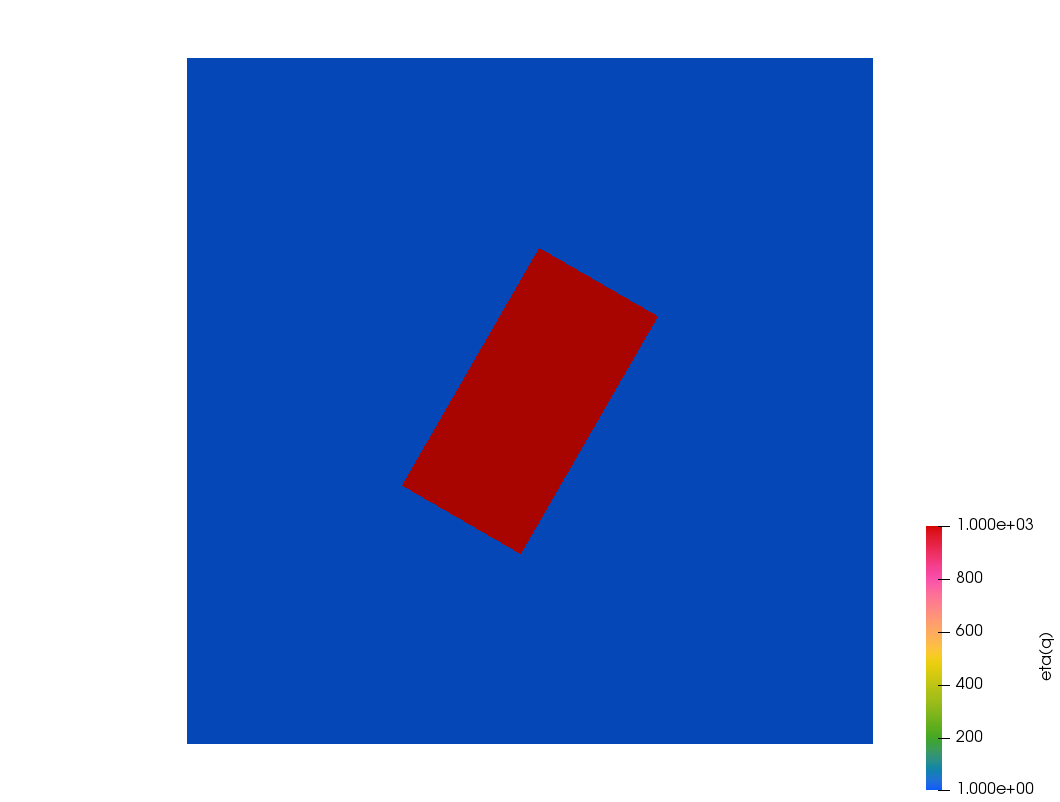
\includegraphics[width=5.57cm]{python_codes/fieldstone_142/results/case1/eta}\\
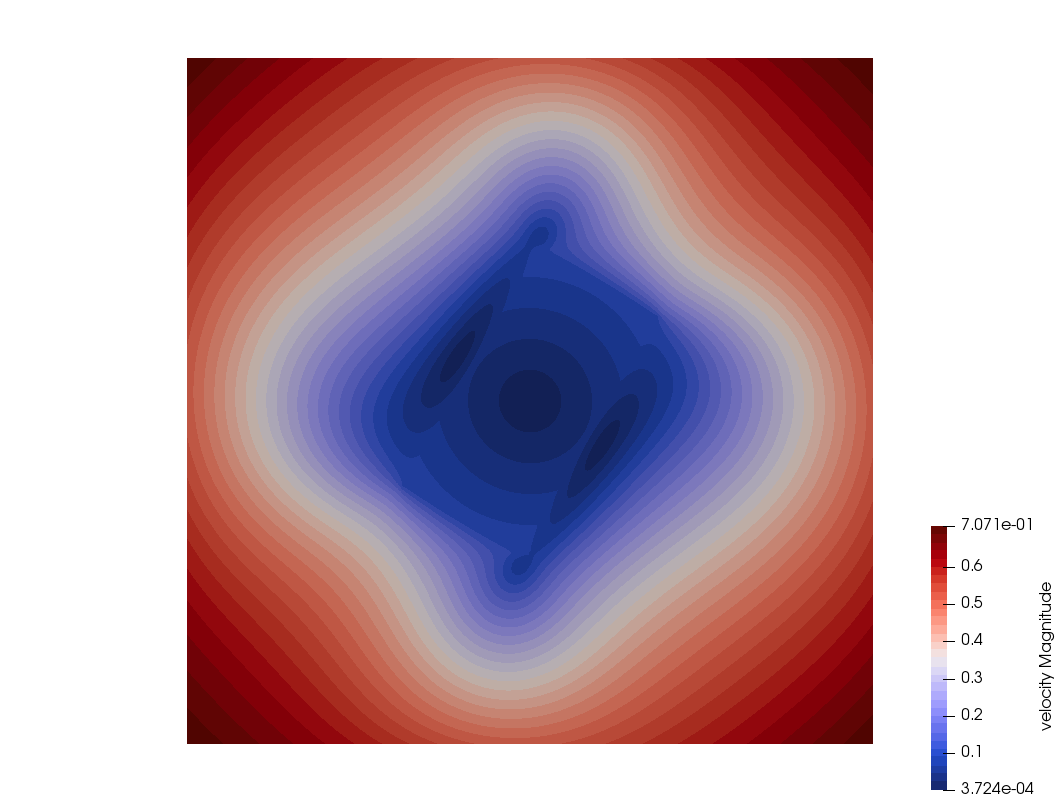
\includegraphics[width=5.57cm]{python_codes/fieldstone_142/results/case1/vel1}
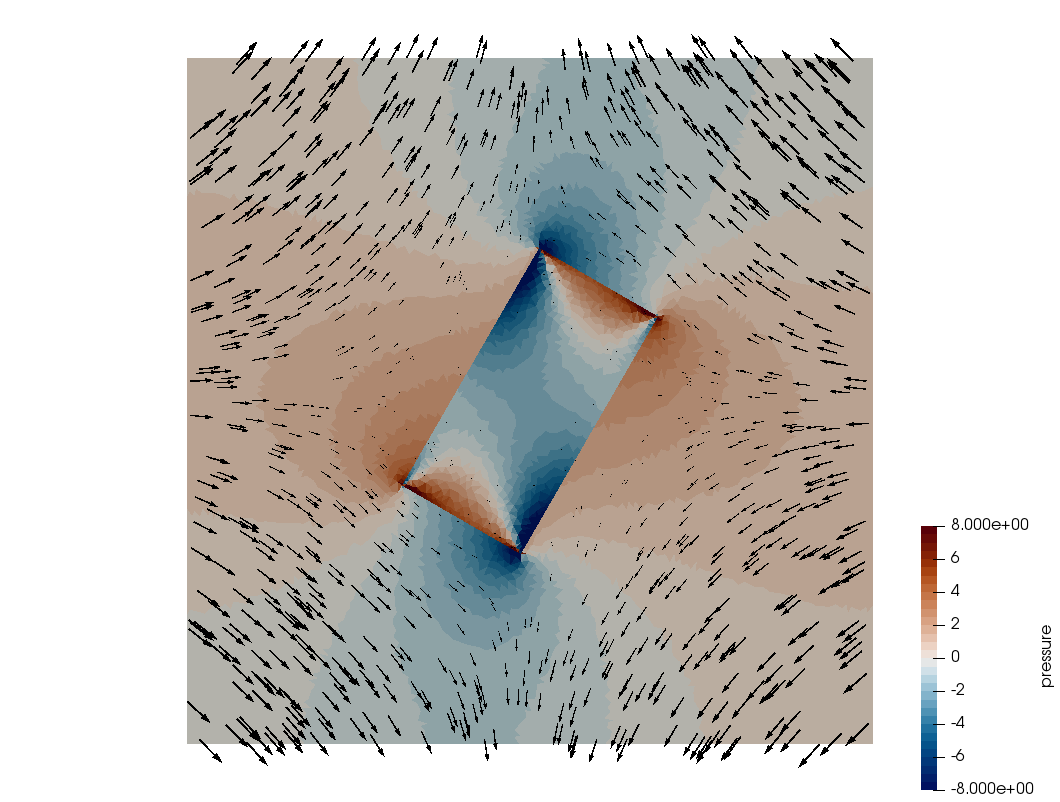
\includegraphics[width=5.57cm]{python_codes/fieldstone_142/results/case1/press1}
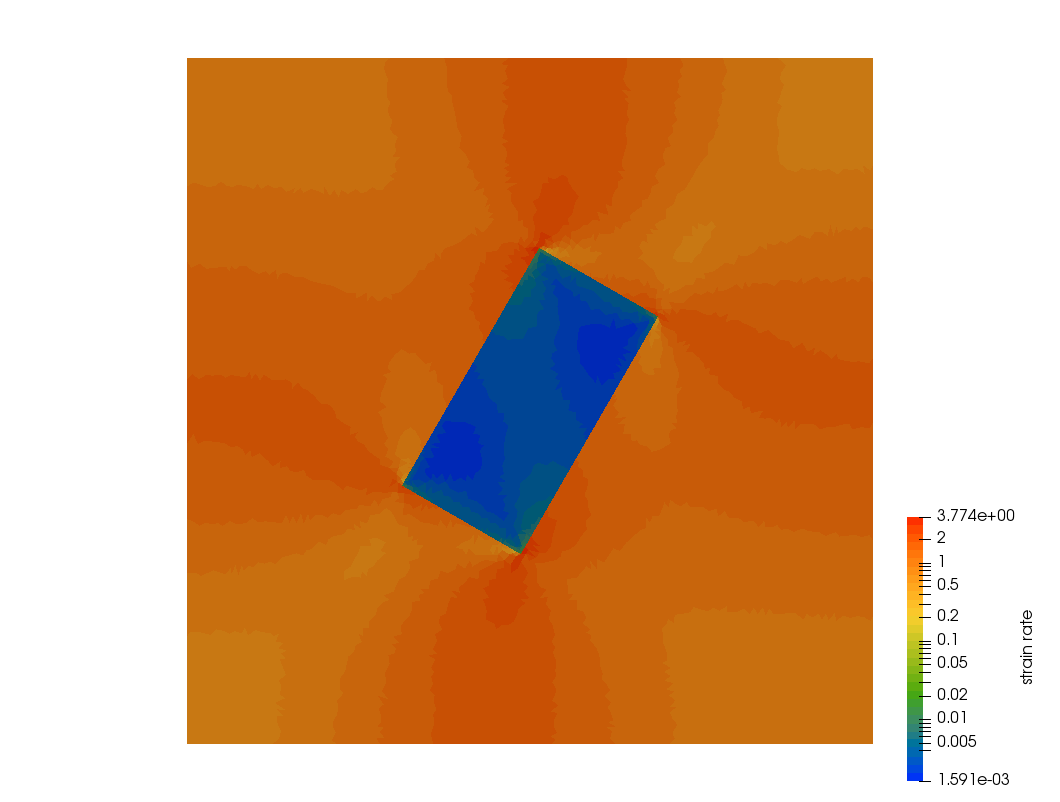
\includegraphics[width=5.57cm]{python_codes/fieldstone_142/results/case1/sr1}\\
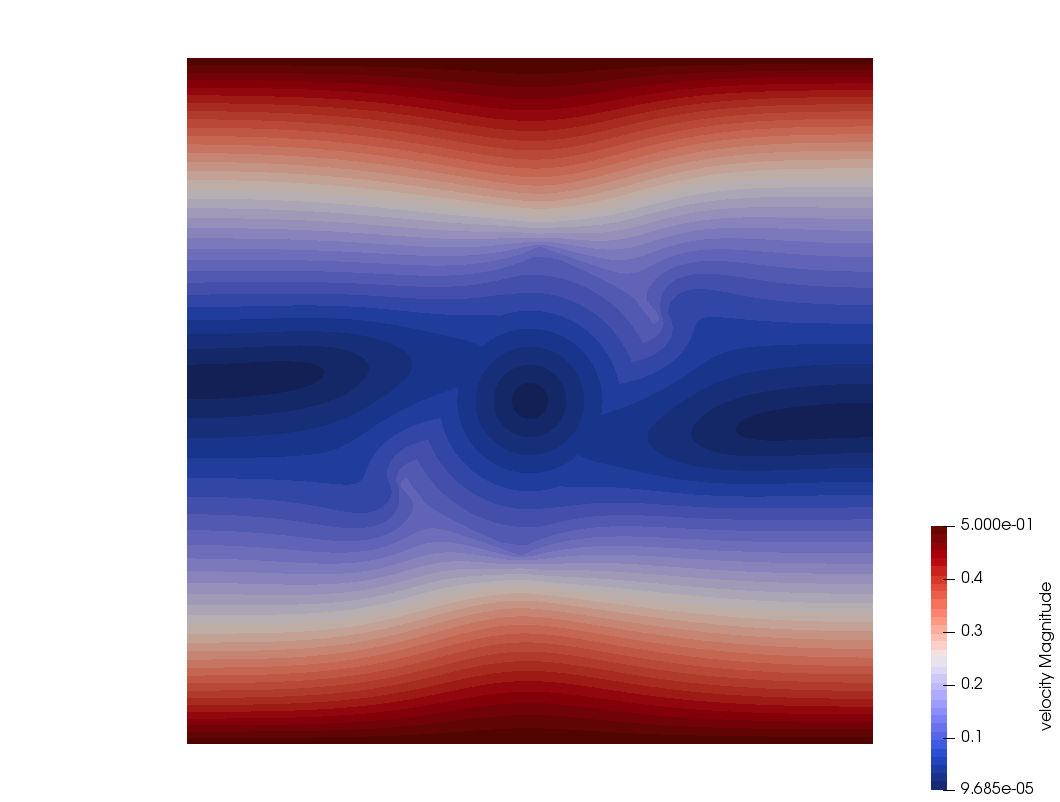
\includegraphics[width=5.57cm]{python_codes/fieldstone_142/results/case1/vel2}
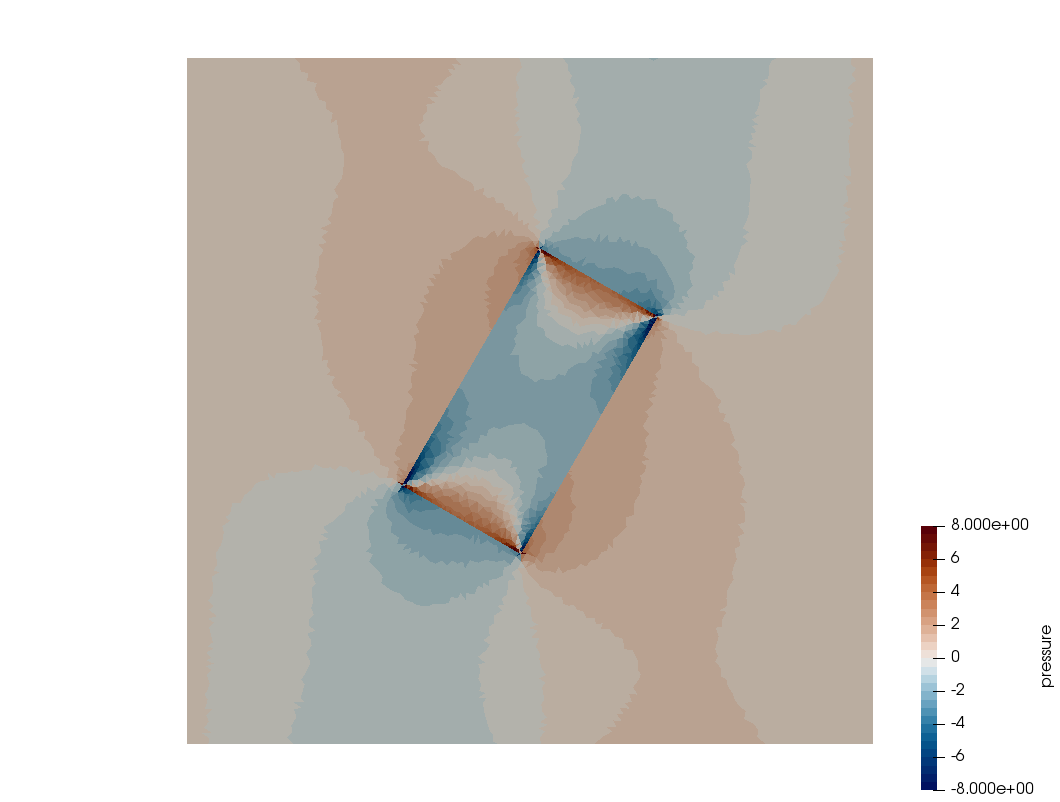
\includegraphics[width=5.57cm]{python_codes/fieldstone_142/results/case1/press2}
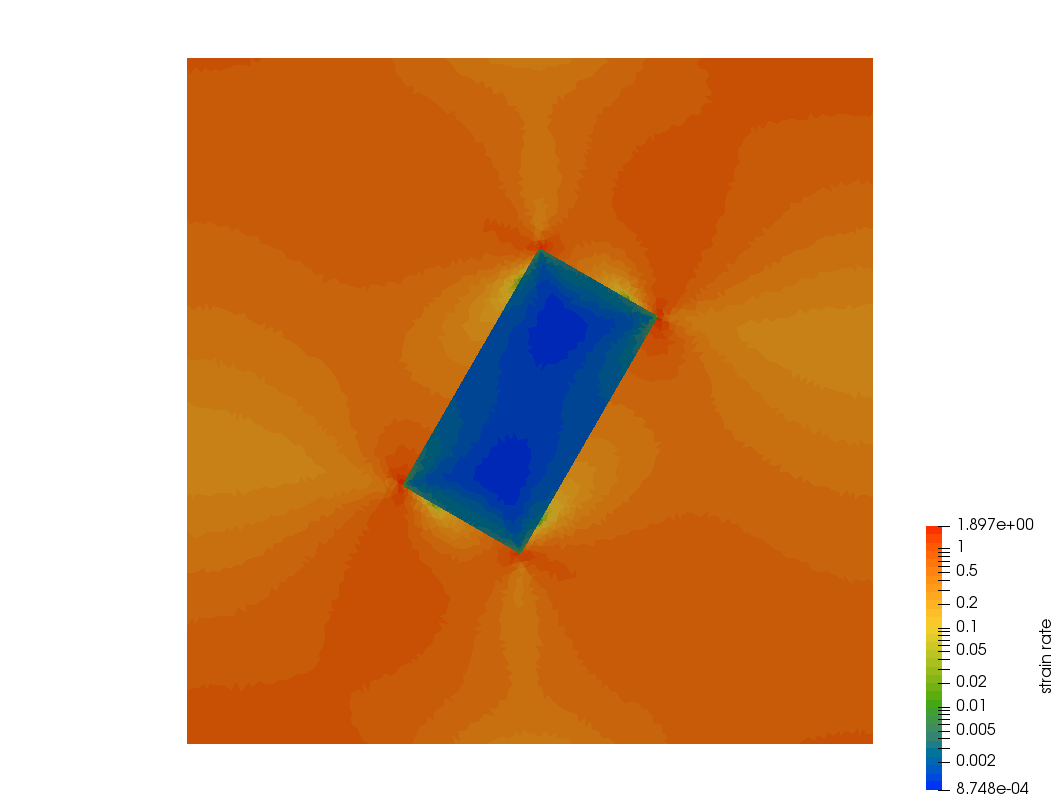
\includegraphics[width=5.57cm]{python_codes/fieldstone_142/results/case1/sr2}\\
{\captionfont In order to favor comparison with the figure of the paper I for once
use a different pressure colorscale ('vik') than normal. 
Second line is Pure Shear (PS), third line is simple shear (SS).}
\end{center}

To validate the results of this stone further, I have run this model with the \aspect
code, and my results agree nicely with those of \aspect:

\begin{center}
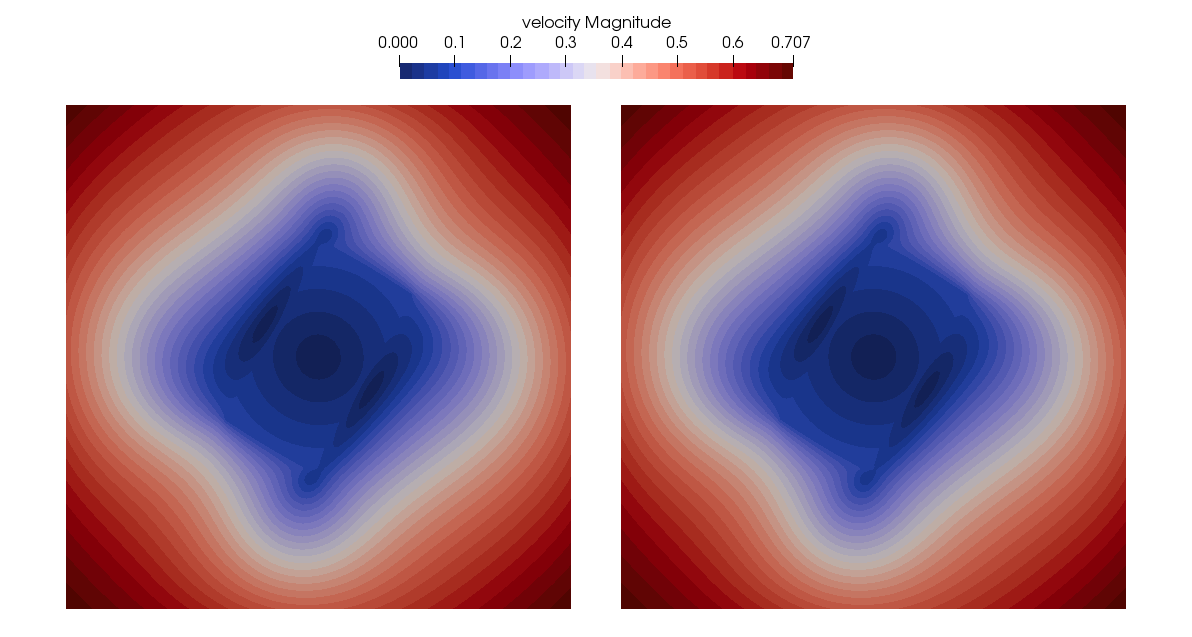
\includegraphics[width=8cm]{python_codes/fieldstone_142/results/case1/aspect/vel}\\
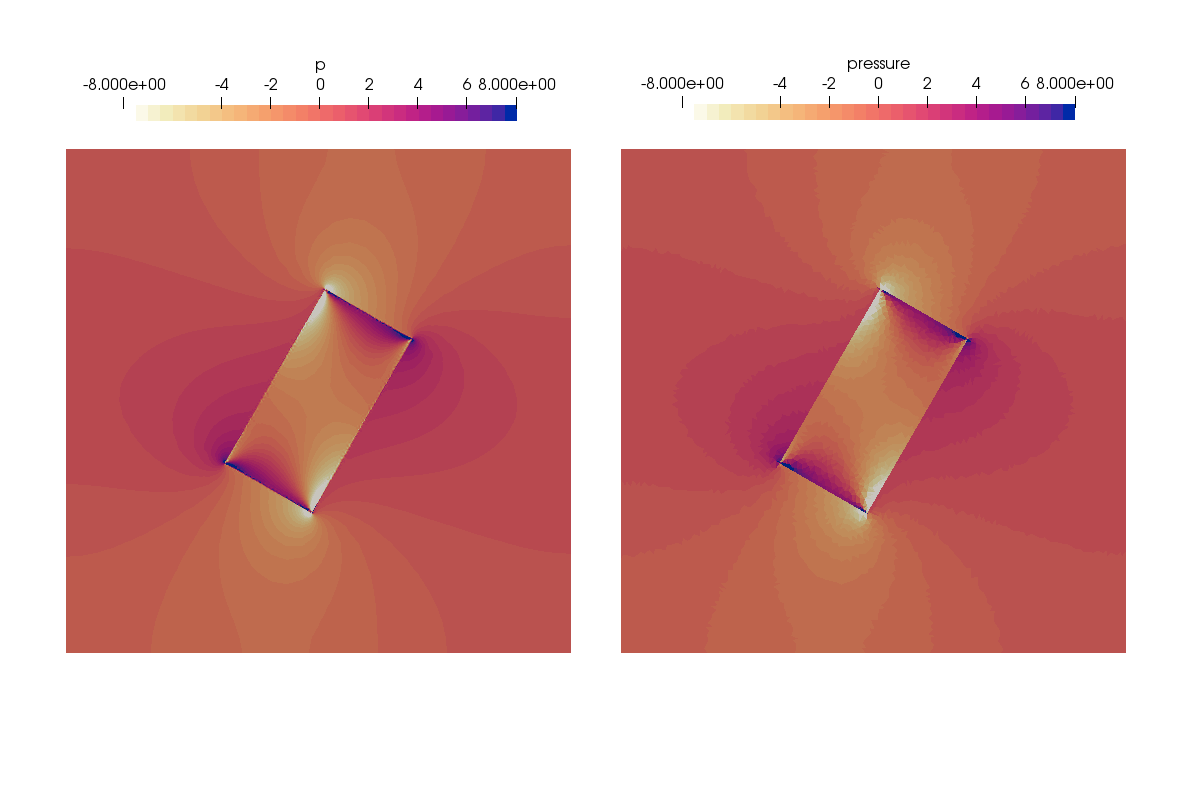
\includegraphics[width=8cm]{python_codes/fieldstone_142/results/case1/aspect/press}\\
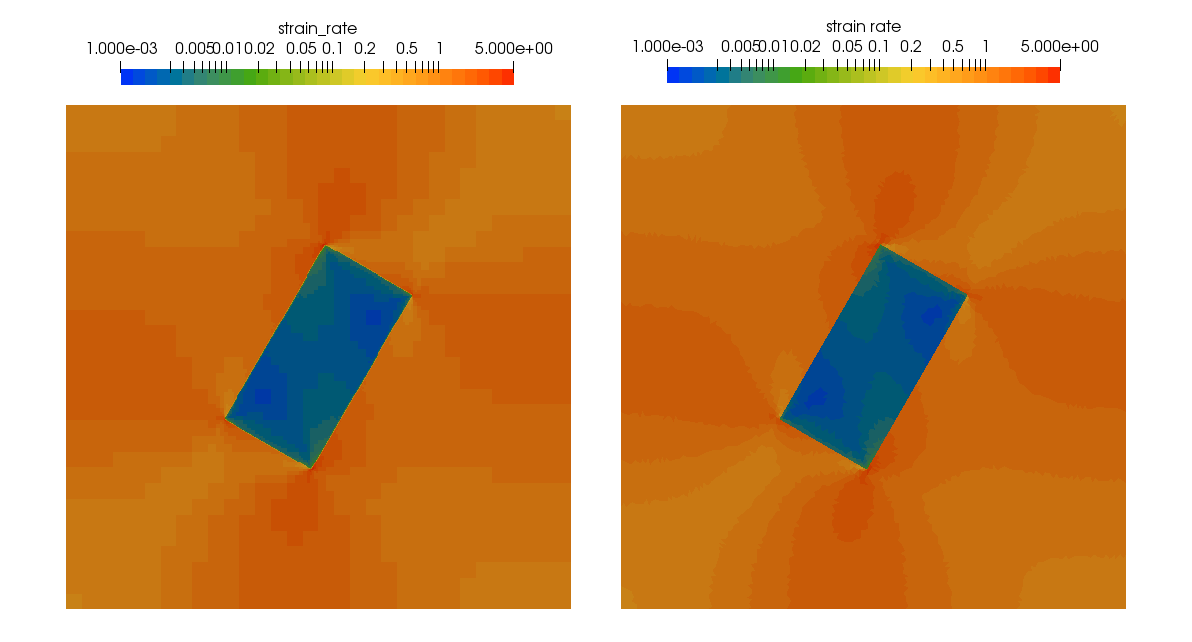
\includegraphics[width=8cm]{python_codes/fieldstone_142/results/case1/aspect/sr}\\
{\captionfont Left: \aspect results; Right: fieldstone results.}
\end{center}


Plotting the \aspect and fieldstone results with a similar
color scale yields the unescapable conclusion that {\color{red} the pressure field 
in the figure of the paper is wrong inside the inclusion}:
\begin{center}
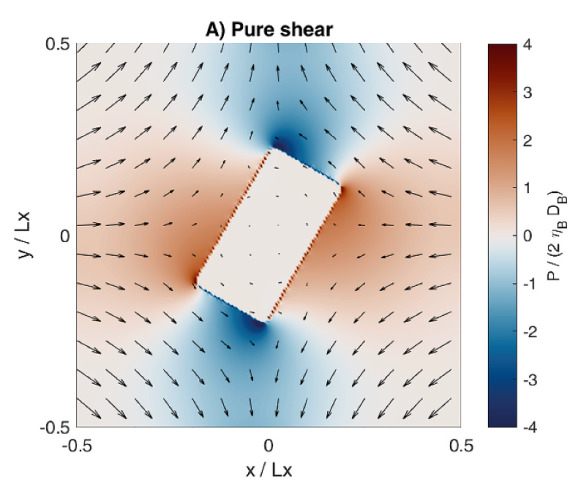
\includegraphics[height=5cm]{python_codes/fieldstone_142/images/hams22_cc}
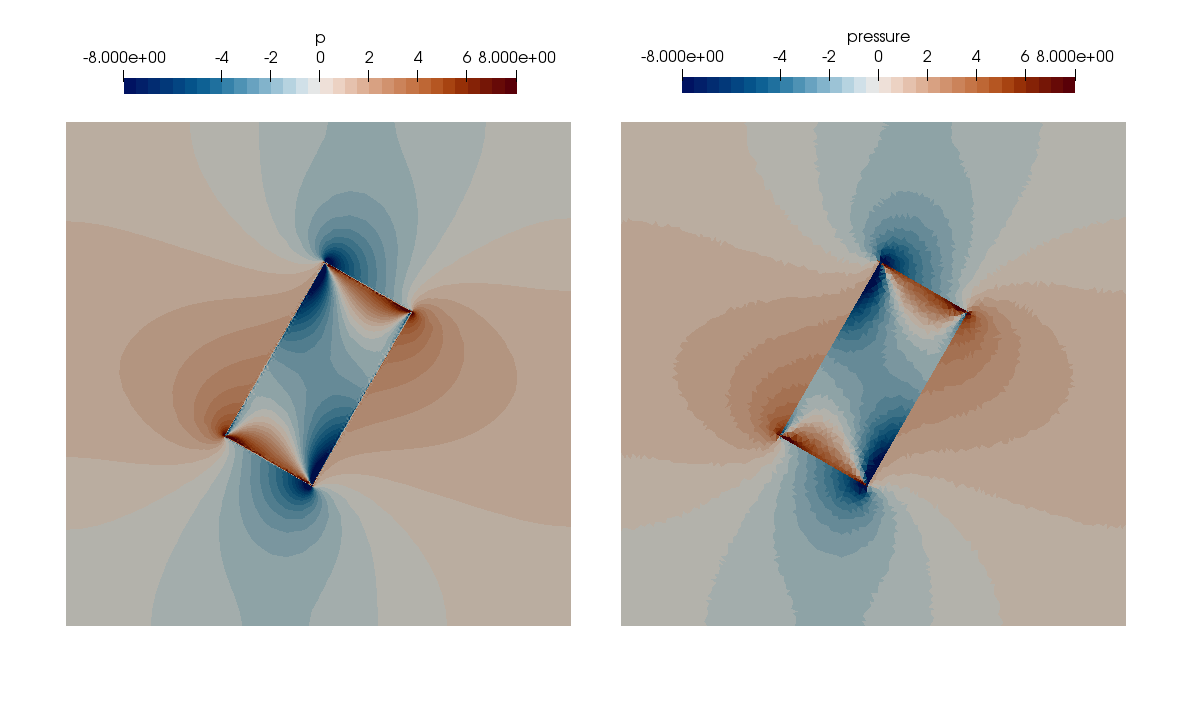
\includegraphics[height=5.6cm]{python_codes/fieldstone_142/results/case1/aspect/press2}\\
{\captionfont In the paper $\eta_B=1$ and $D_B=1$ so that the pressure range in their
figure is in fact [-8:8].i Left: fig 6 of the paper; Middle: \aspect; Right: fieldstone.}
\end{center}

\newpage
%%%%%%%%%%%%%%%%%%%%%%%%%%%%%%%%%%%%%%%%%%%%%%%%%%%%%%%%%%%%%%%%%%%%%%%%%%%%%%%%%%%%%%%%%%5
\section*{Case 2: Power-law viscous matrix and weak elliptical inclusion}


\begin{center}
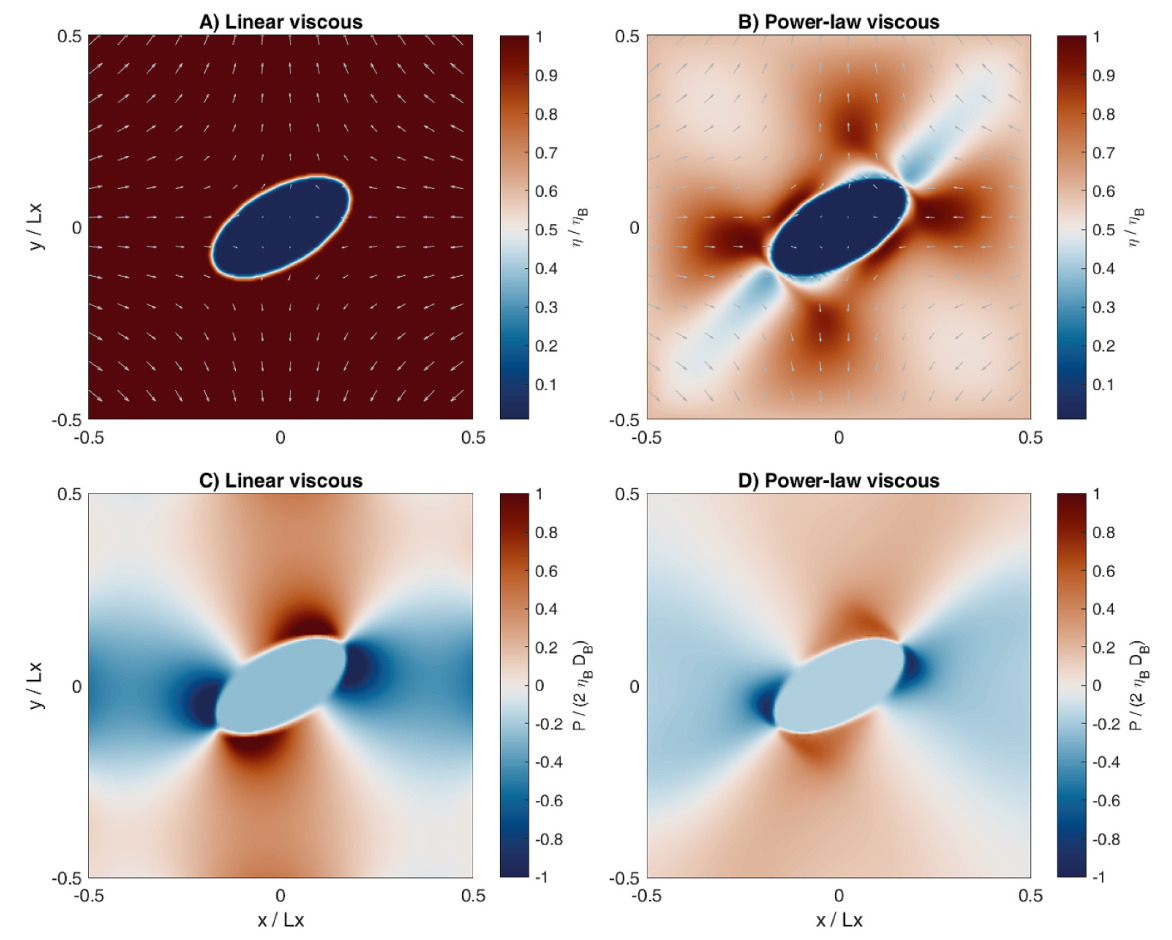
\includegraphics[width=8.5cm]{python_codes/fieldstone_142/images/hams22_d}
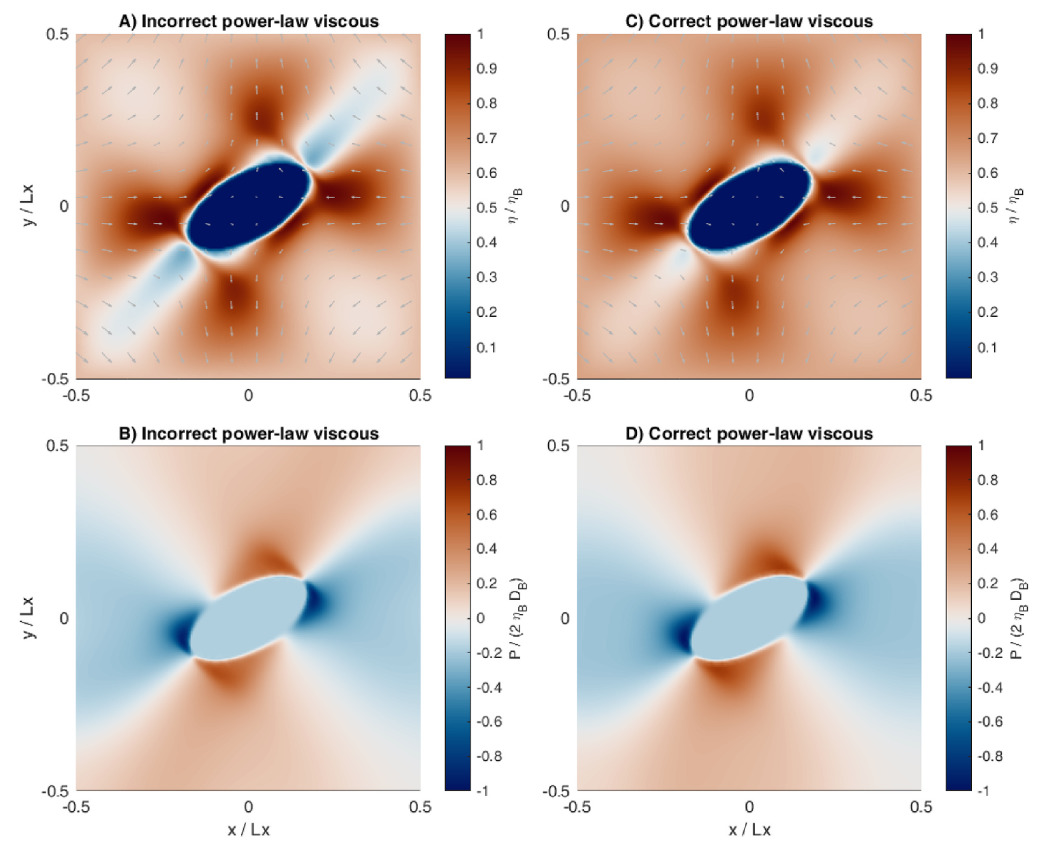
\includegraphics[width=8.5cm]{python_codes/fieldstone_142/images/hams22_dd}\\
\captionfont{Taken from \cite{hams22}.
Viscosity and pressure field of a
weak (viscosity ratio of 1000) elliptical inclusion under pure shear. A model with a
purely linear viscosity (left panels) is compared against a model with an effective
viscosity including power-law viscosity (right panels). The power-law viscosity is
calculated using a stress exponent of 5 and a constant reference stress of 1.5 (see equation
(12)). The arrows display the velocity field, they are not to scale and only for direction.
The ellipse’s semi-major axis is twice as long as its semi-minor axis and corresponds to 0.2
times the model width. The semi-major axis is rotated by 30 degrees from the horizontal axis.}
\end{center}

The paper comes with two corrected Matlab and Octave codes that are available online under
\url{https://github.com/halterw/A_simple_computer_program}.
I have run the Octave version as is (I do not have Matlab).
Rather annoyingly, it runs, shows results every 2000 iterations, ultimately converges
but does not produce a plot. Also there is no visualisation of velocity? 

\begin{center}
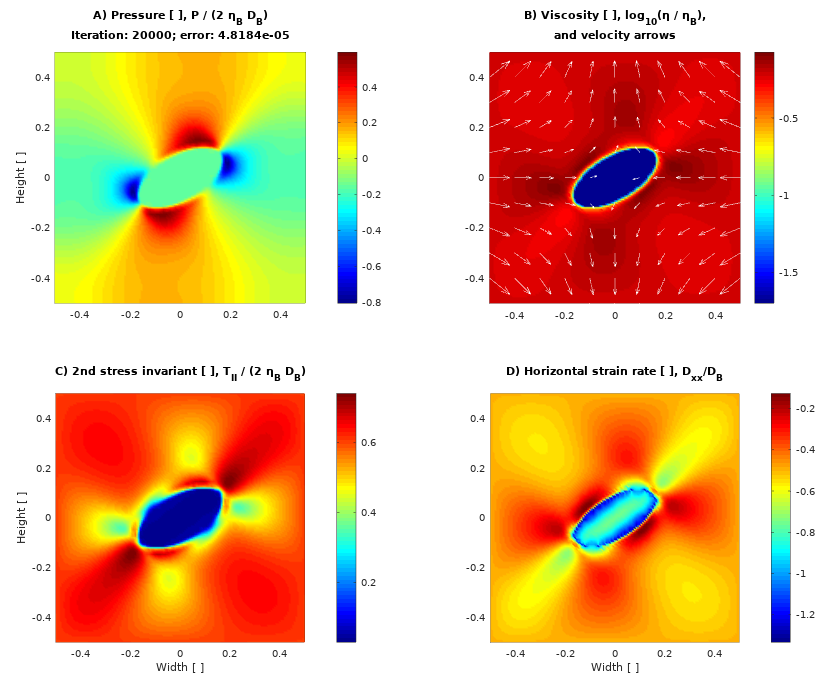
\includegraphics[width=12cm]{python_codes/fieldstone_142/images/octave1}\\
{\captionfont Screen capture of the Octave code output when run as is off github.}
\end{center}

I have therefore modified the code to add velocity visualisation and export to png.
I have also removed the normalisation of results.
If I now set \verb|n_exp=1| with a 1000 viscosity ratio the model now becomes Newtonian,
but the code fails to converge. After more than 200,000 iterations the results are as 
follows:

\begin{center}
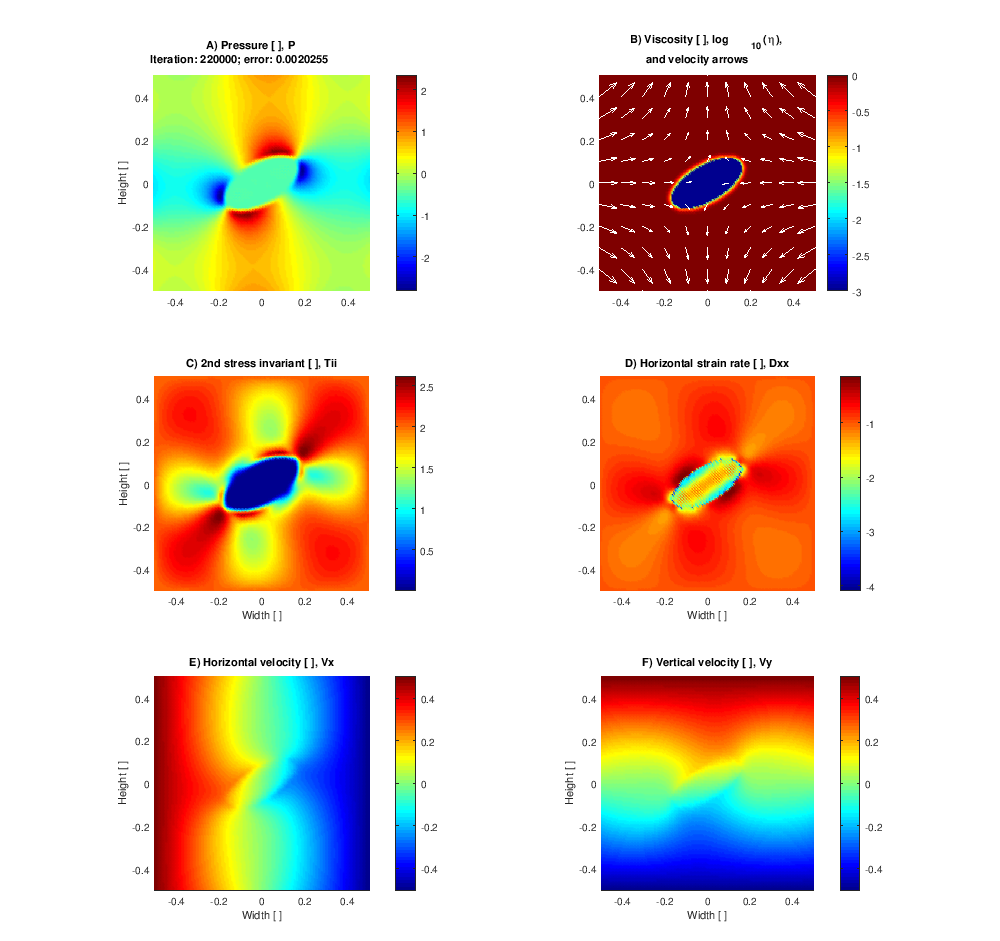
\includegraphics[width=13cm]{python_codes/fieldstone_142/images/octave2}\\
{\captionfont Screen capture of the Octave code output for a viscosity ratio of 1000.
Modified output. Dxx looks somewhat suspicious...}
\end{center}

As it turns out, when one lets the code run for a {\it long} time, 
the error looks like:
\begin{center}
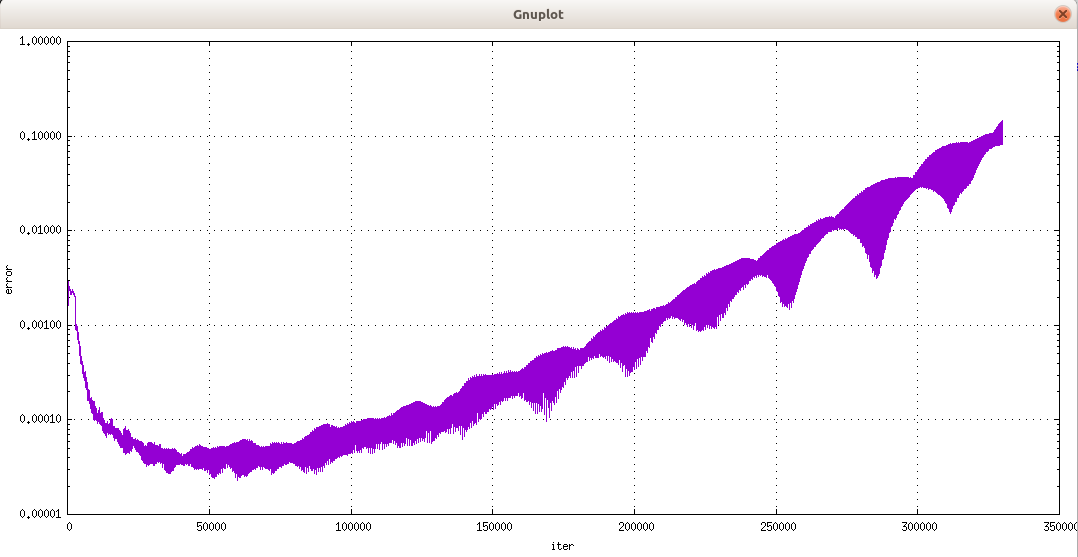
\includegraphics[width=8cm]{python_codes/fieldstone_142/results/case2/error}
\end{center}
In summary, {\color{red} the solver is not converging} and the results above are meaningless!


\begin{center}
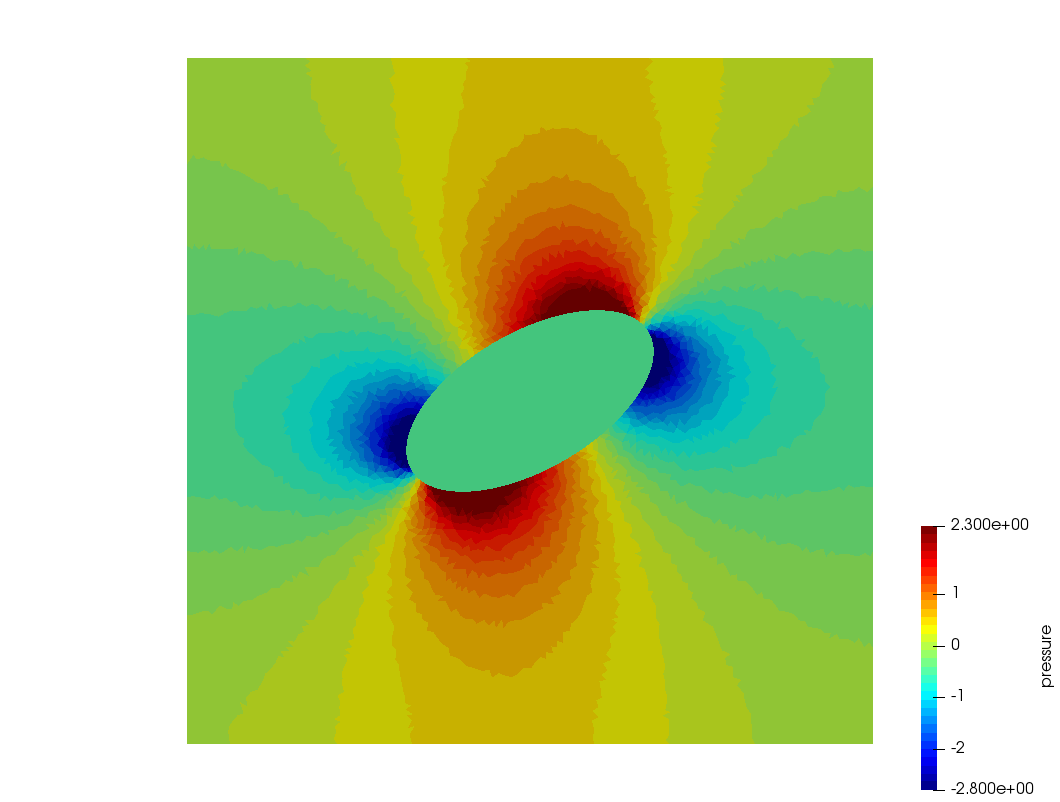
\includegraphics[width=5.7cm]{python_codes/fieldstone_142/results/case2/press2}
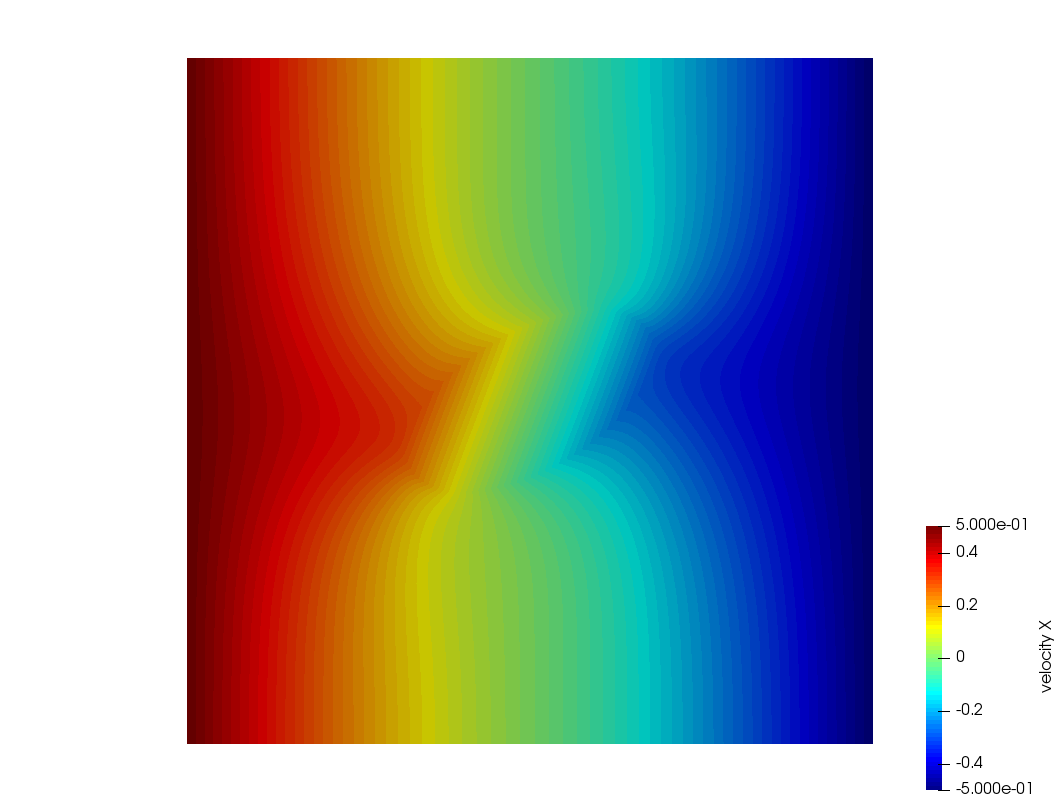
\includegraphics[width=5.7cm]{python_codes/fieldstone_142/results/case2/u2}
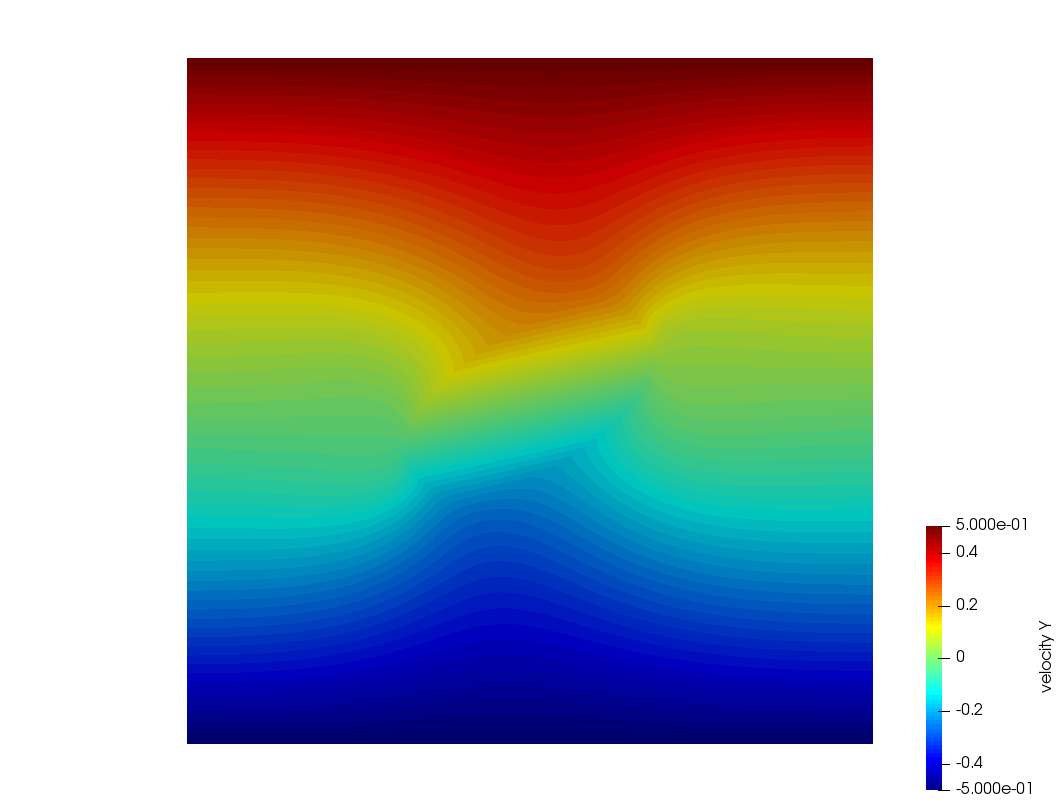
\includegraphics[width=5.7cm]{python_codes/fieldstone_142/results/case2/v2}\\
{\captionfont I get a reasonable match for pressure and velocity - provided I use 
the same colorscale and range.}
\end{center}

\newpage
Here is the full set of fields with appropriate color scales obtained with 
this \stone:
\begin{center}
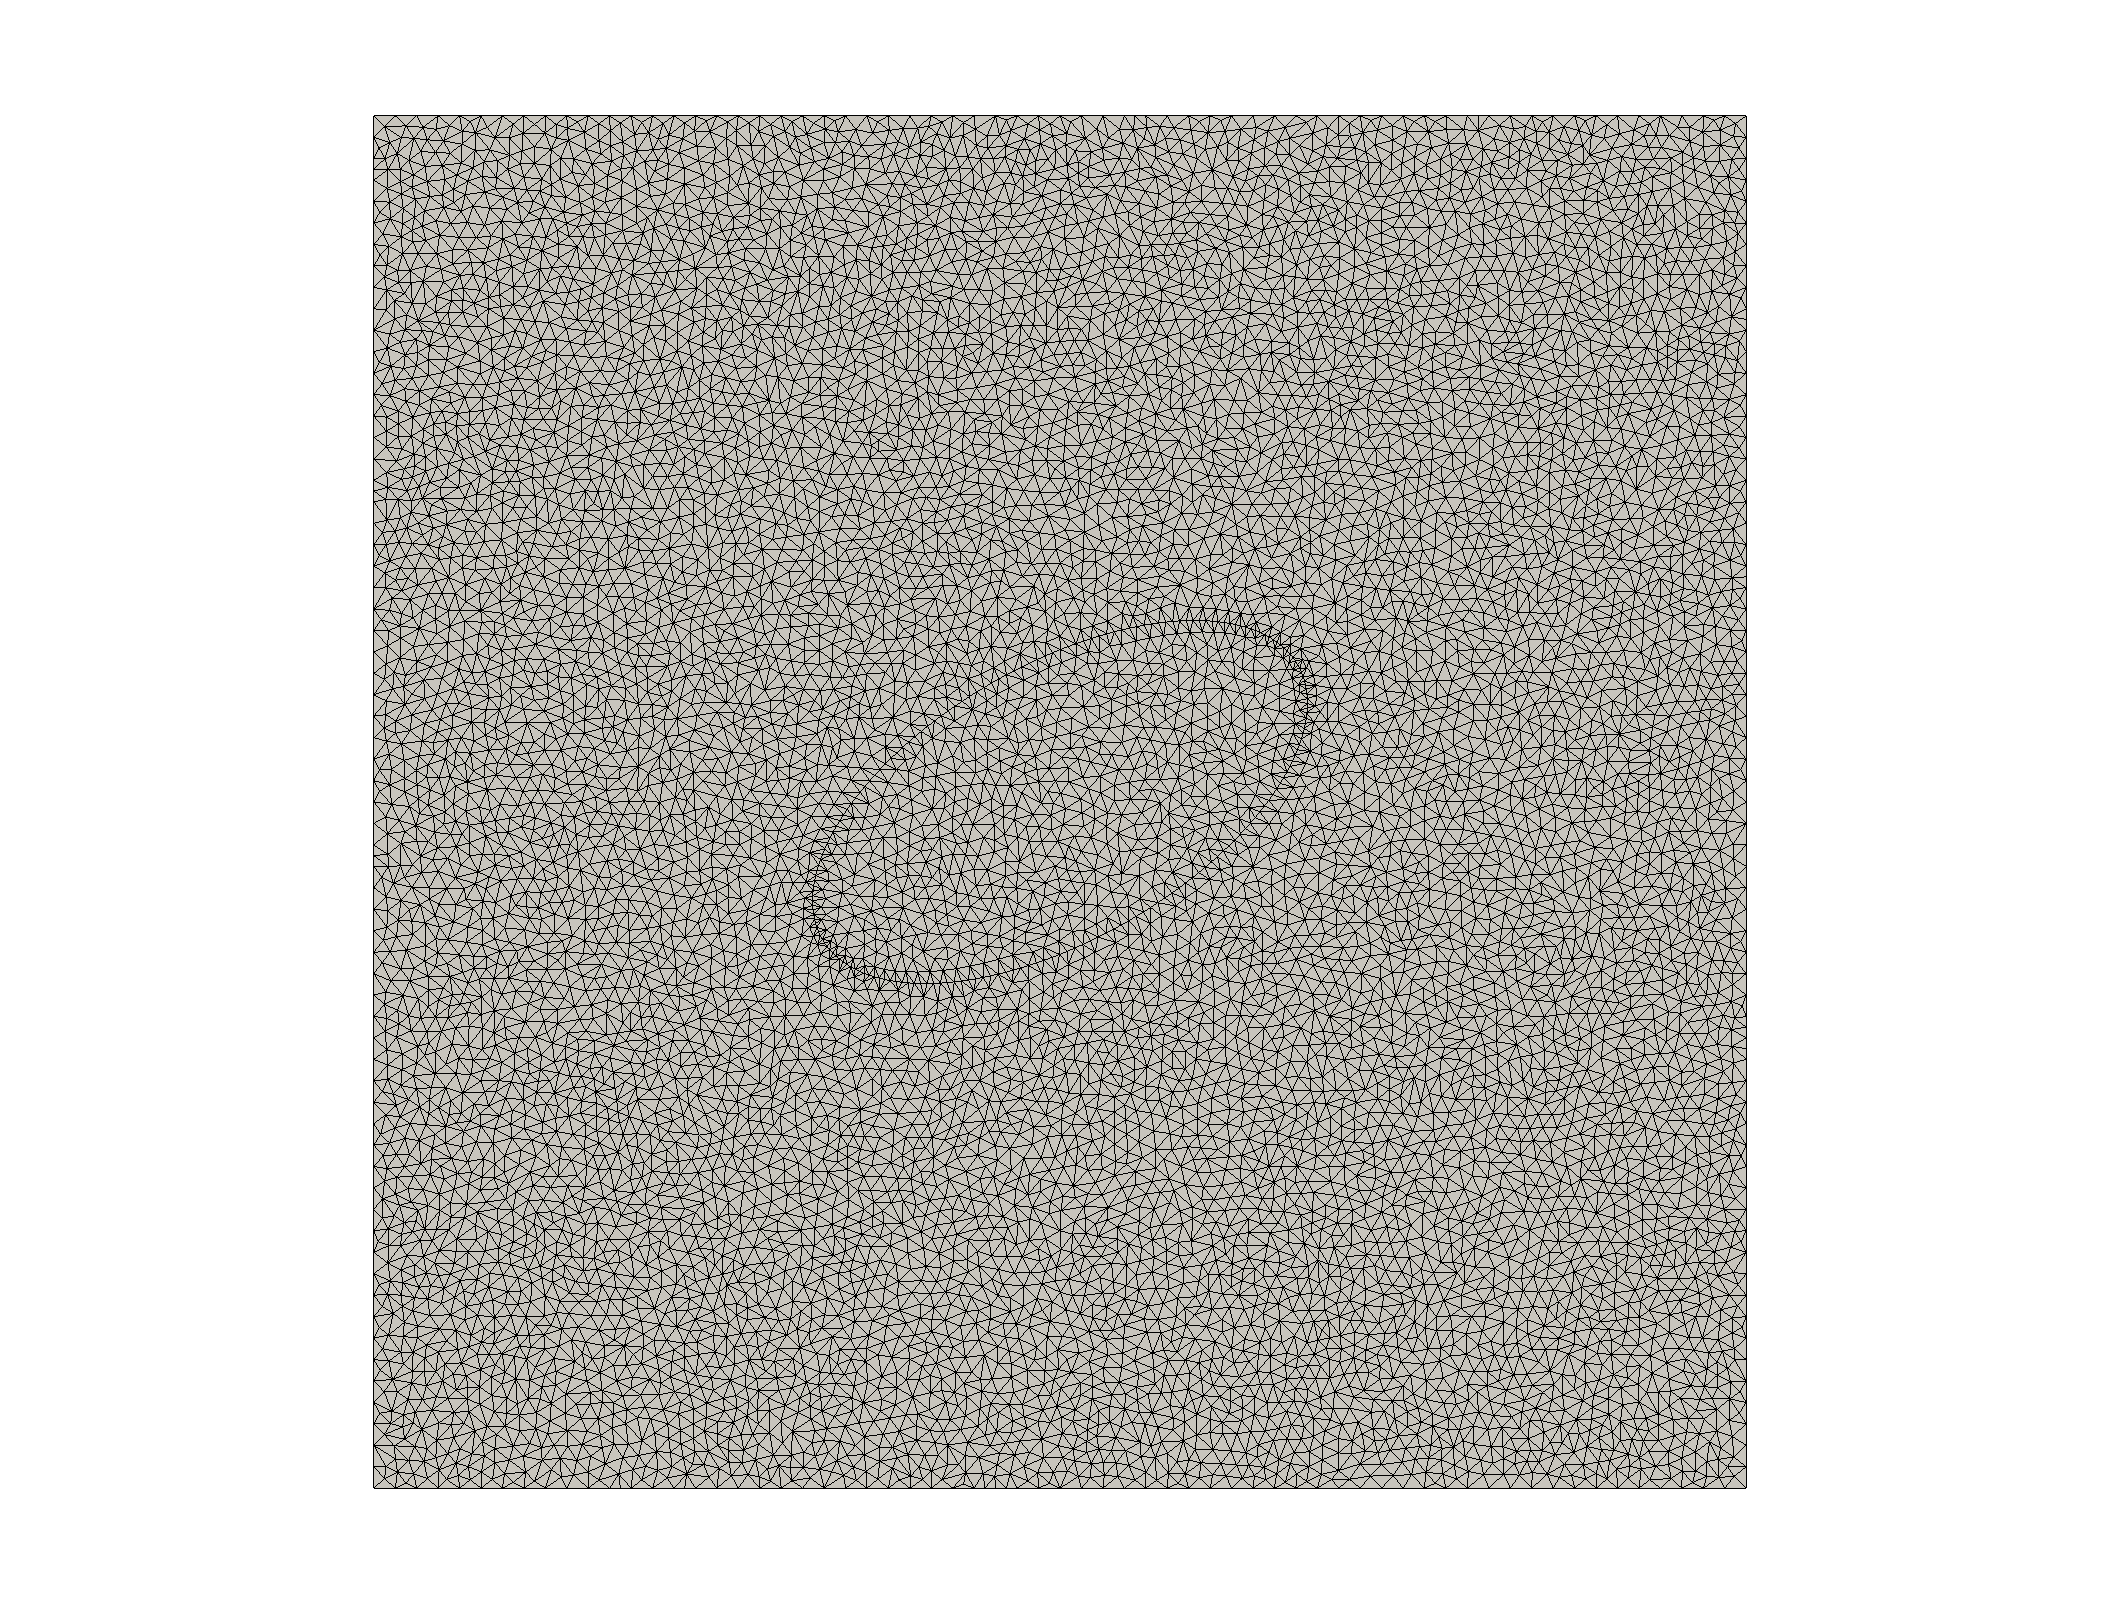
\includegraphics[width=5.57cm]{python_codes/fieldstone_142/results/case2/mesh}
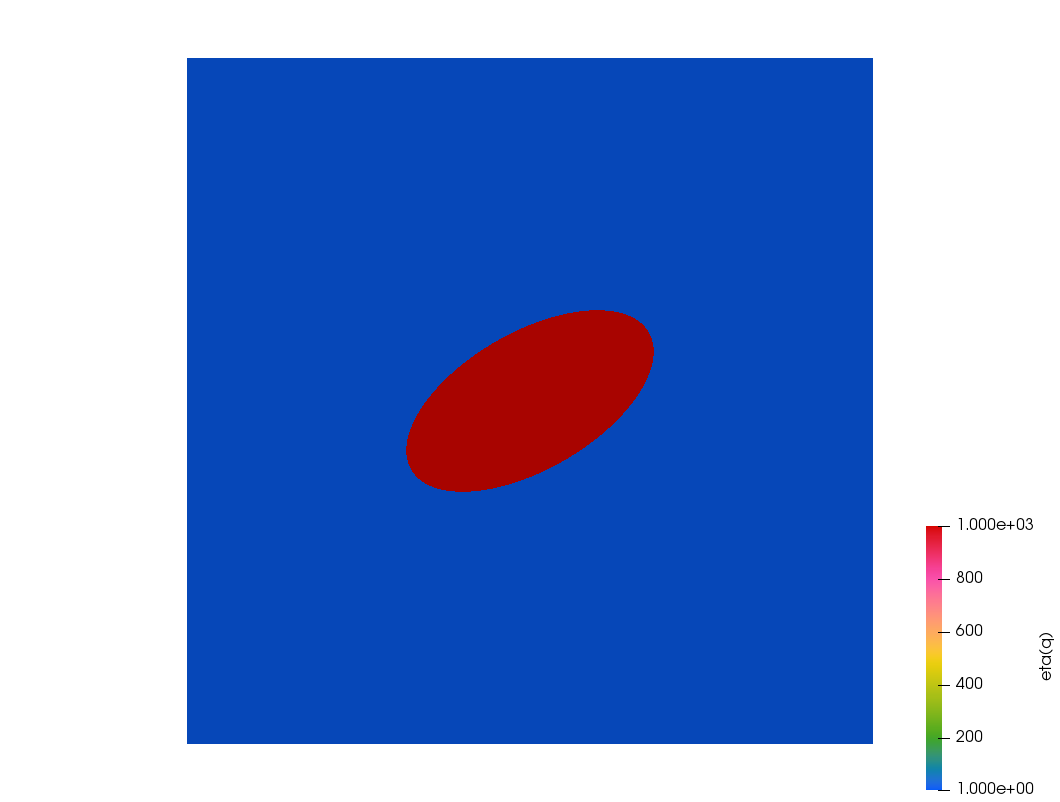
\includegraphics[width=5.57cm]{python_codes/fieldstone_142/results/case2/eta}\\
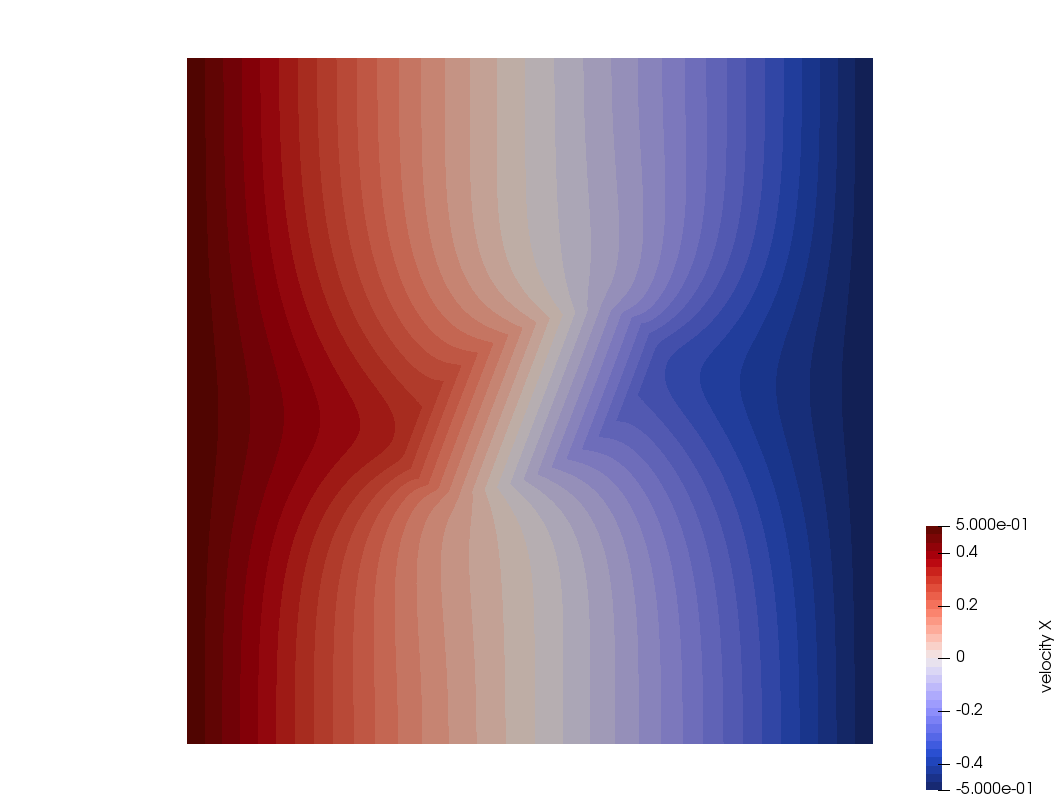
\includegraphics[width=5.57cm]{python_codes/fieldstone_142/results/case2/u}
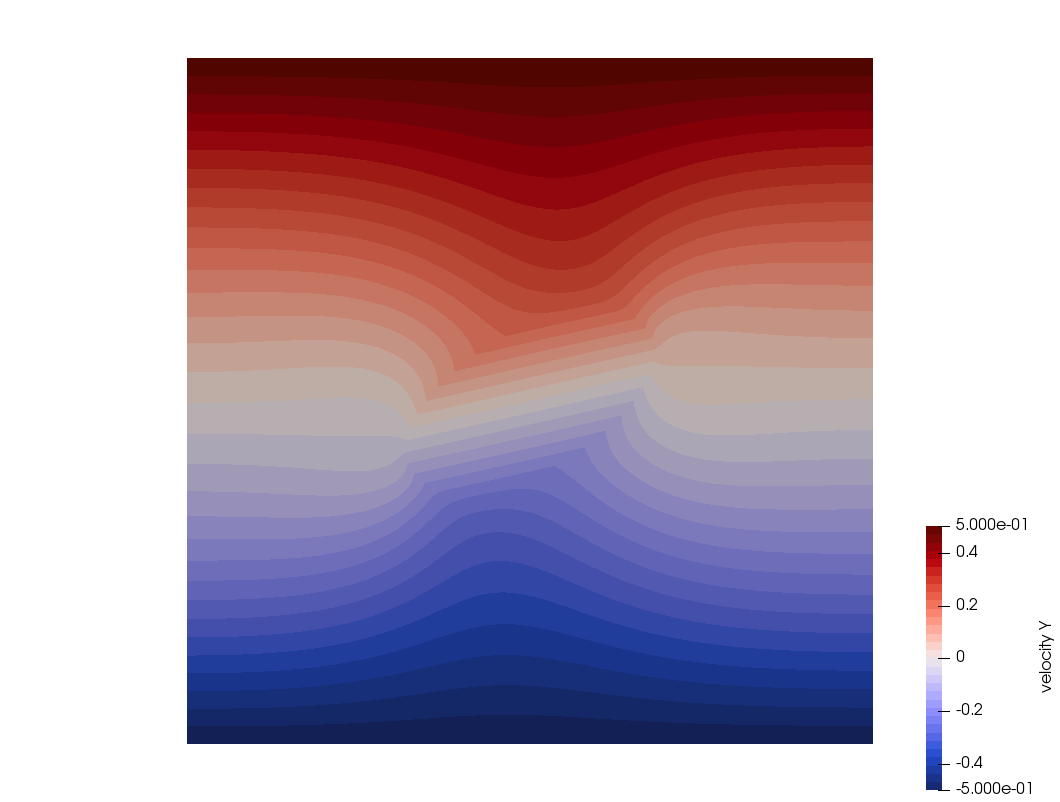
\includegraphics[width=5.57cm]{python_codes/fieldstone_142/results/case2/v}
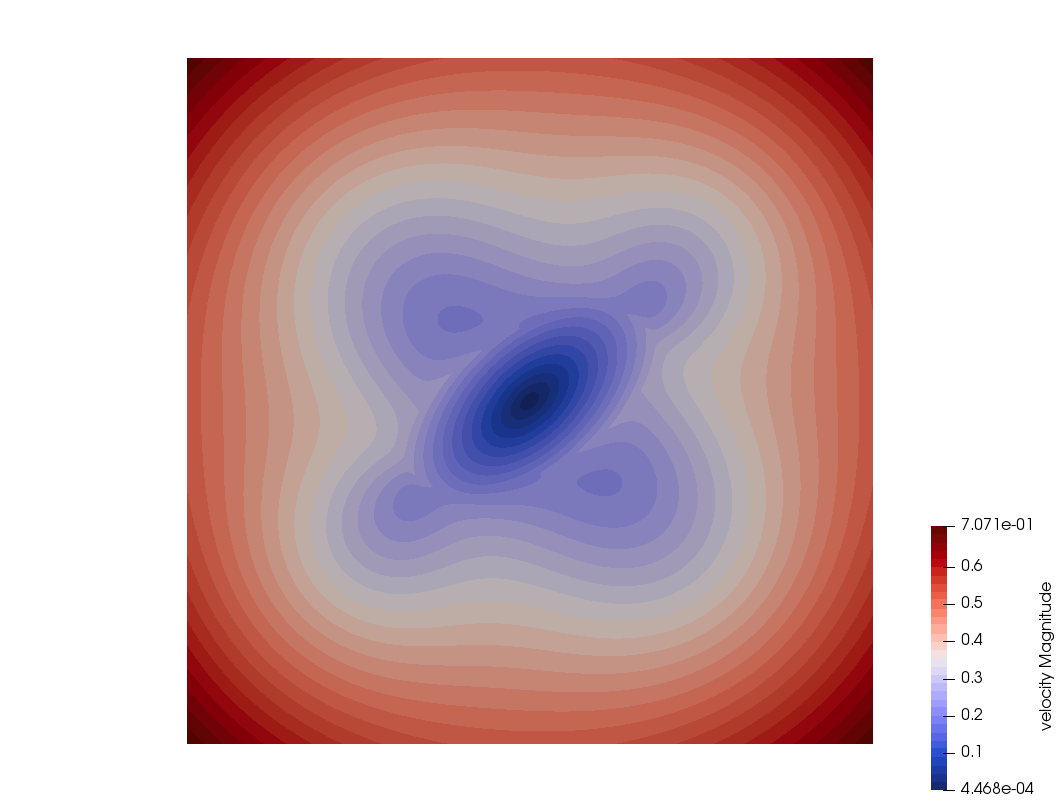
\includegraphics[width=5.57cm]{python_codes/fieldstone_142/results/case2/vel}\\
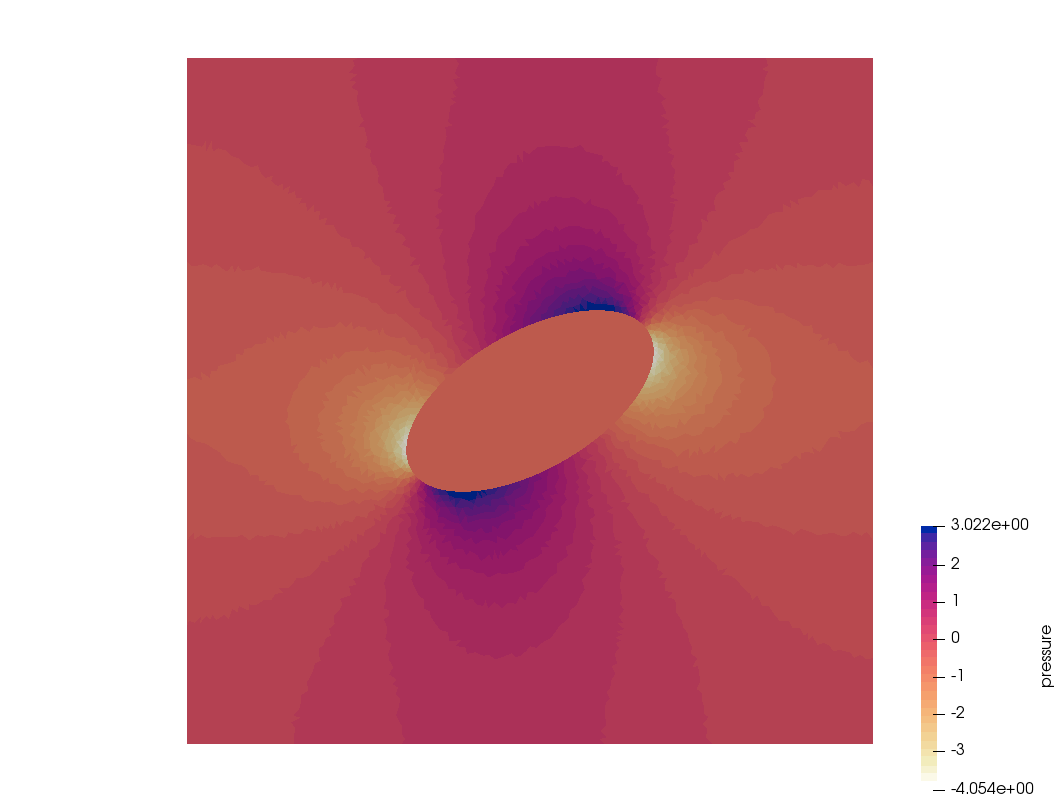
\includegraphics[width=5.57cm]{python_codes/fieldstone_142/results/case2/press}
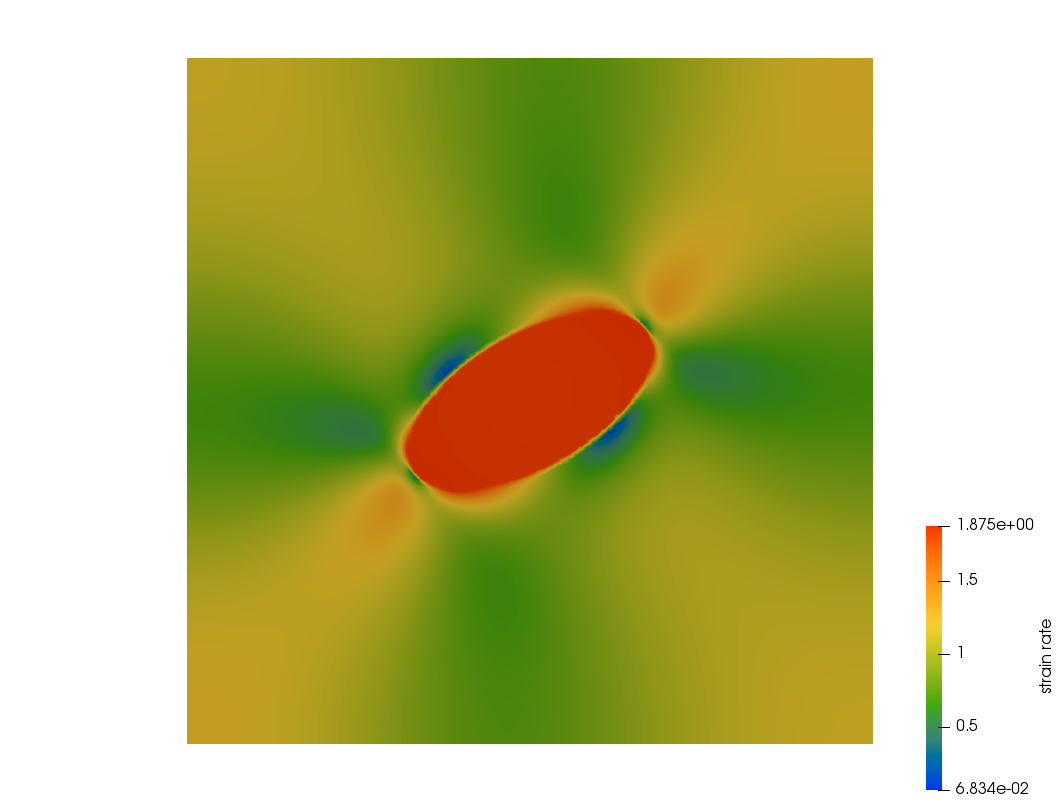
\includegraphics[width=5.57cm]{python_codes/fieldstone_142/results/case2/sr}
\end{center}

To validate the results of this stone further, I have run this model with the \aspect
code:

\begin{center}
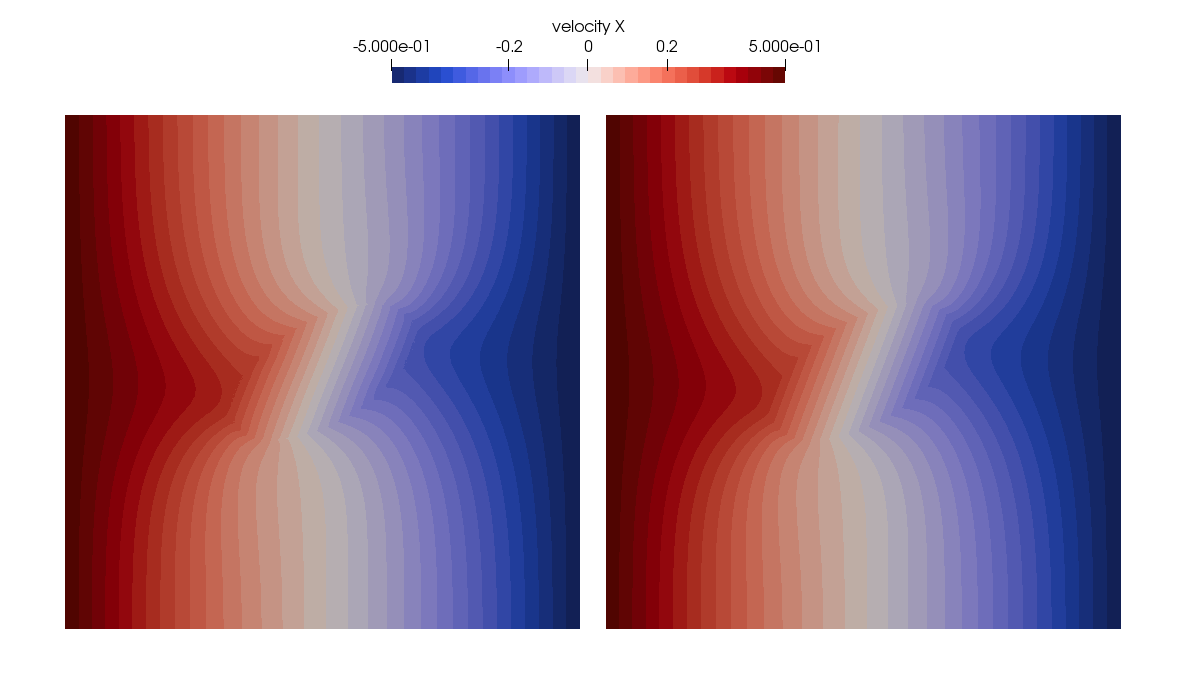
\includegraphics[width=8cm]{python_codes/fieldstone_142/results/case2/aspect/u}
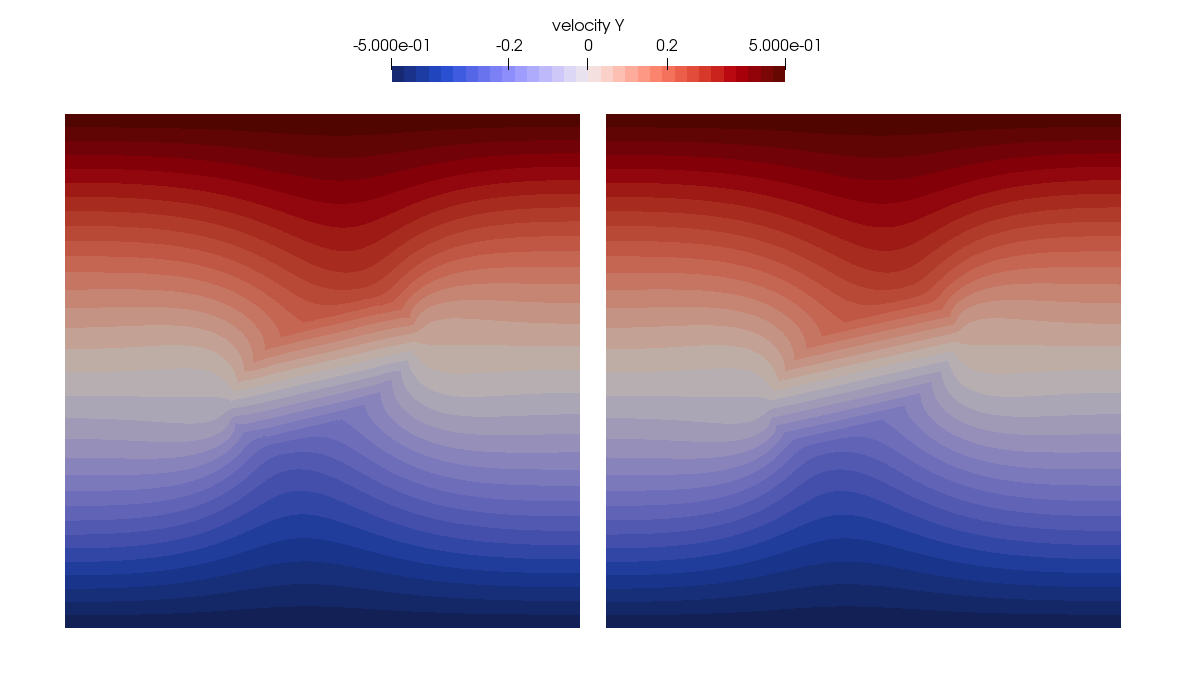
\includegraphics[width=8cm]{python_codes/fieldstone_142/results/case2/aspect/v}\\
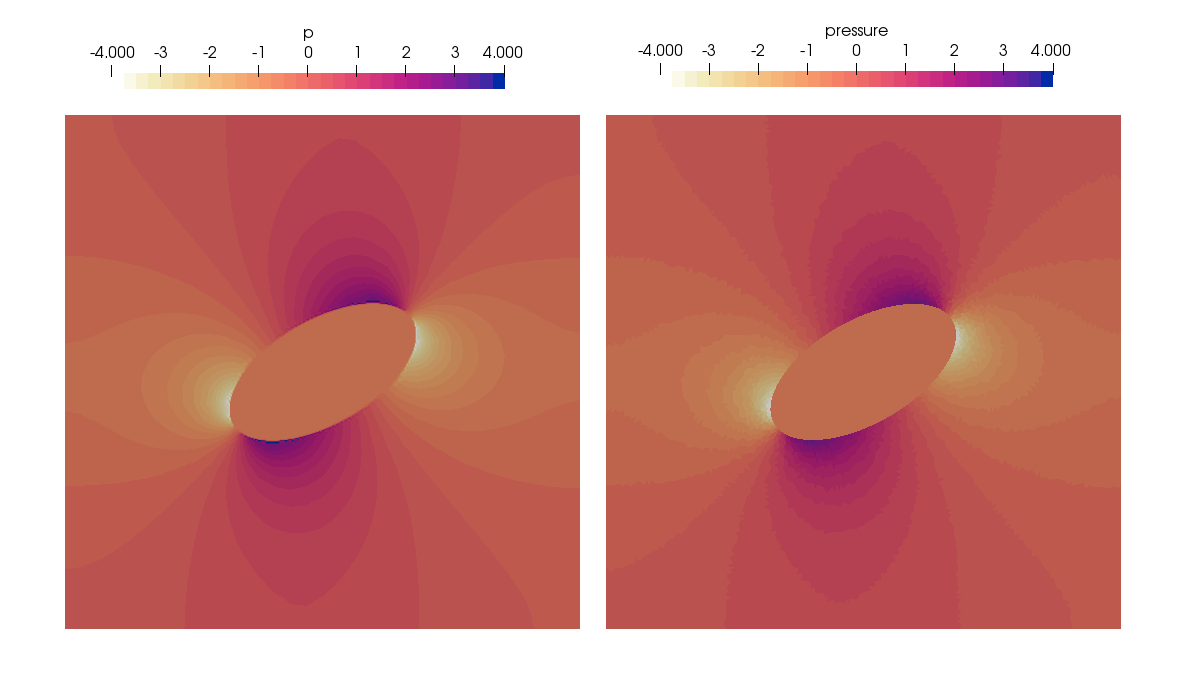
\includegraphics[width=8cm]{python_codes/fieldstone_142/results/case2/aspect/press}
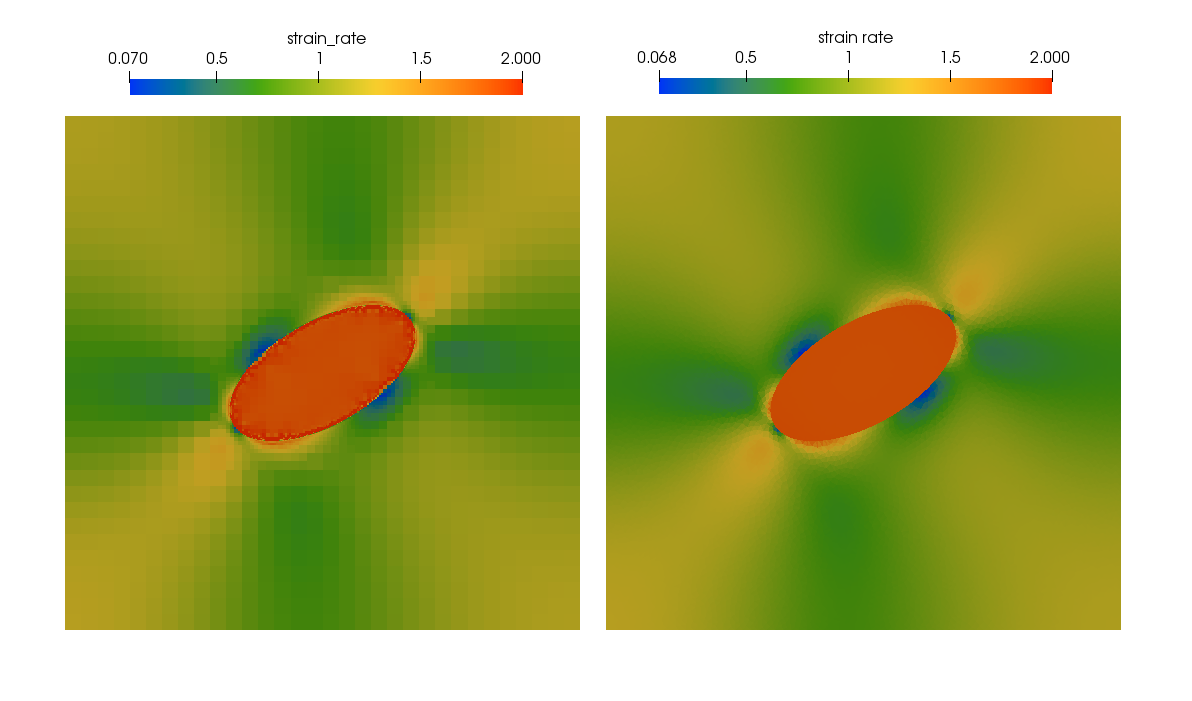
\includegraphics[width=8cm]{python_codes/fieldstone_142/results/case2/aspect/sr}\\
{\captionfont Left: \aspect results; Right: fieldstone results.}
\end{center}


\newpage
%%%%%%%%%%%%%%%%%%%%%%%%%%%%%%%%%%%%%%%%%%%%%%%%%%%%%%%%%%%%%%%%%%%%%%%%%%%%%%%%%%%%%%%%%%5
\section*{Exp4: Multiple inclusions of different shape}

\begin{center}
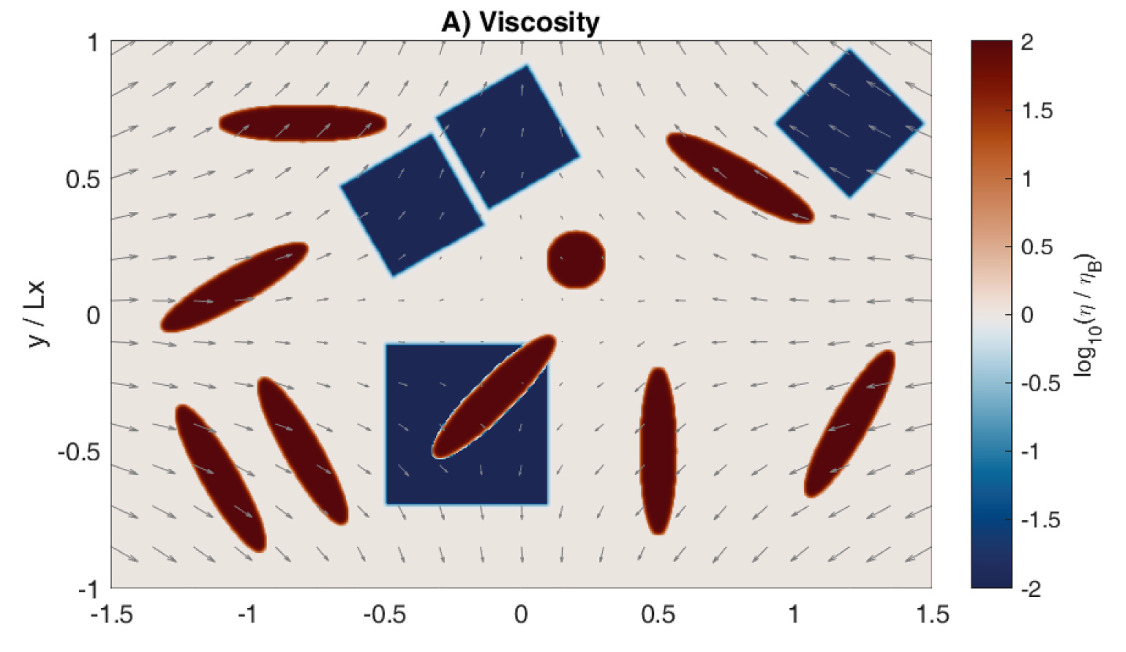
\includegraphics[width=8cm]{python_codes/fieldstone_142/images/hams22_e}
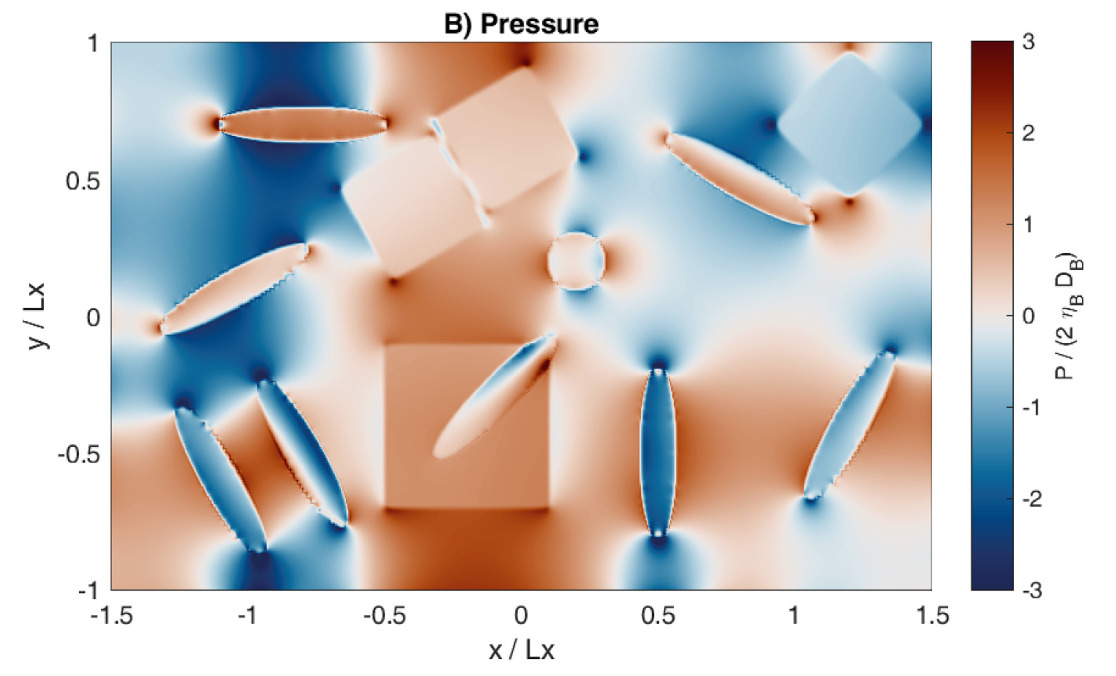
\includegraphics[width=8cm]{python_codes/fieldstone_142/images/hams22_f}\\
\captionfont{
Viscosity and pressure for a combination of different geometrical weak and strong inclusions 
subjected to horizontally compressive pure shear. The arrows in
panel A) display the velocity field, they are not to scale and only for direction. 
The ellipses are 100 times more viscous, the squares are 100 times less viscous than the
surrounding matrix. Except for the circular inclusion, all ellipses possess the same aspect ratio.
}
\end{center}



%%%%%%%%%%%%%%%%%%%%%%%%%%%%%%%%%%%%%%%%%%%%%%%%%%%%%%%%%%%%%%%%%%%%%%%%%%%%%%%%%%%%%%%%%%5
\section*{Exp5: Inclusion with a more natural shape}


\begin{center}
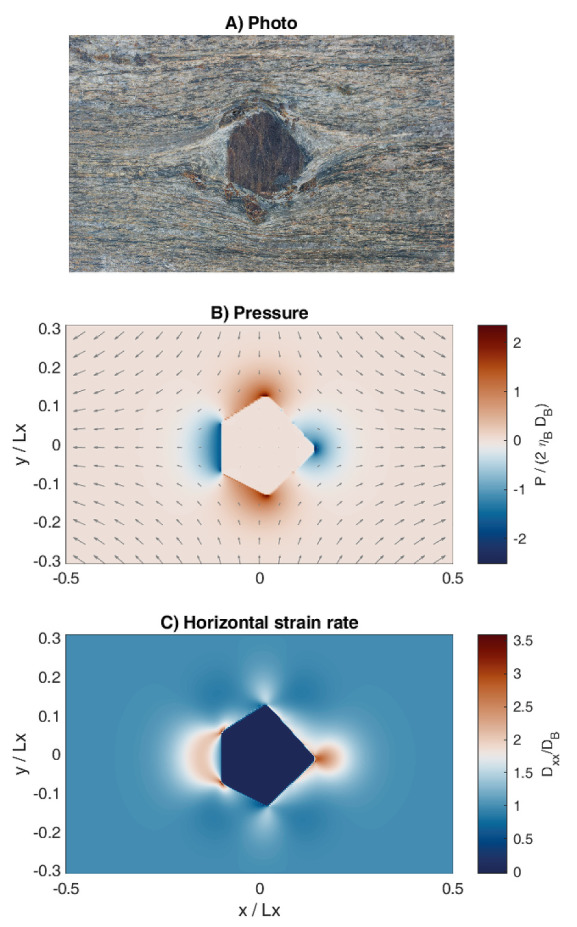
\includegraphics[width=8cm]{python_codes/fieldstone_142/images/hams22_g}\\
\captionfont{
Numerical modelling of the pressure and strain rate field around a
garnet inclusion using a photo from an actual inclusion (Fig. 1 C). In the model
the strong inclusion has a viscosity contrast of 1000 and is subjected to horizontally 
extensional pure shear. The garnet was redrawn as a polygon using the
Matlab ginput function. The arrows in panel B) display the velocity field, they
are not to scale and only for direction.
}
\end{center}







